% Generated by Sphinx.
\def\sphinxdocclass{report}
\documentclass[letterpaper,10pt,english]{sphinxmanual}
\usepackage[utf8]{inputenc}
\DeclareUnicodeCharacter{00A0}{\nobreakspace}
\usepackage{cmap}
\usepackage[T1]{fontenc}
\usepackage{babel}
\usepackage{times}
\usepackage[Bjarne]{fncychap}
\usepackage{longtable}
\usepackage{sphinx}
\usepackage{multirow}


\title{Candy Basket Documentation}
\date{January 30, 2015}
\release{1.0}
\author{Ghislain Hachey, Maya Goldman and Dan McGarry}
\newcommand{\sphinxlogo}{}
\renewcommand{\releasename}{Release}
\makeindex

\makeatletter
\def\PYG@reset{\let\PYG@it=\relax \let\PYG@bf=\relax%
    \let\PYG@ul=\relax \let\PYG@tc=\relax%
    \let\PYG@bc=\relax \let\PYG@ff=\relax}
\def\PYG@tok#1{\csname PYG@tok@#1\endcsname}
\def\PYG@toks#1+{\ifx\relax#1\empty\else%
    \PYG@tok{#1}\expandafter\PYG@toks\fi}
\def\PYG@do#1{\PYG@bc{\PYG@tc{\PYG@ul{%
    \PYG@it{\PYG@bf{\PYG@ff{#1}}}}}}}
\def\PYG#1#2{\PYG@reset\PYG@toks#1+\relax+\PYG@do{#2}}

\expandafter\def\csname PYG@tok@gd\endcsname{\def\PYG@tc##1{\textcolor[rgb]{0.63,0.00,0.00}{##1}}}
\expandafter\def\csname PYG@tok@gu\endcsname{\let\PYG@bf=\textbf\def\PYG@tc##1{\textcolor[rgb]{0.50,0.00,0.50}{##1}}}
\expandafter\def\csname PYG@tok@gt\endcsname{\def\PYG@tc##1{\textcolor[rgb]{0.00,0.27,0.87}{##1}}}
\expandafter\def\csname PYG@tok@gs\endcsname{\let\PYG@bf=\textbf}
\expandafter\def\csname PYG@tok@gr\endcsname{\def\PYG@tc##1{\textcolor[rgb]{1.00,0.00,0.00}{##1}}}
\expandafter\def\csname PYG@tok@cm\endcsname{\let\PYG@it=\textit\def\PYG@tc##1{\textcolor[rgb]{0.25,0.50,0.56}{##1}}}
\expandafter\def\csname PYG@tok@vg\endcsname{\def\PYG@tc##1{\textcolor[rgb]{0.73,0.38,0.84}{##1}}}
\expandafter\def\csname PYG@tok@m\endcsname{\def\PYG@tc##1{\textcolor[rgb]{0.13,0.50,0.31}{##1}}}
\expandafter\def\csname PYG@tok@mh\endcsname{\def\PYG@tc##1{\textcolor[rgb]{0.13,0.50,0.31}{##1}}}
\expandafter\def\csname PYG@tok@cs\endcsname{\def\PYG@tc##1{\textcolor[rgb]{0.25,0.50,0.56}{##1}}\def\PYG@bc##1{\setlength{\fboxsep}{0pt}\colorbox[rgb]{1.00,0.94,0.94}{\strut ##1}}}
\expandafter\def\csname PYG@tok@ge\endcsname{\let\PYG@it=\textit}
\expandafter\def\csname PYG@tok@vc\endcsname{\def\PYG@tc##1{\textcolor[rgb]{0.73,0.38,0.84}{##1}}}
\expandafter\def\csname PYG@tok@il\endcsname{\def\PYG@tc##1{\textcolor[rgb]{0.13,0.50,0.31}{##1}}}
\expandafter\def\csname PYG@tok@go\endcsname{\def\PYG@tc##1{\textcolor[rgb]{0.20,0.20,0.20}{##1}}}
\expandafter\def\csname PYG@tok@cp\endcsname{\def\PYG@tc##1{\textcolor[rgb]{0.00,0.44,0.13}{##1}}}
\expandafter\def\csname PYG@tok@gi\endcsname{\def\PYG@tc##1{\textcolor[rgb]{0.00,0.63,0.00}{##1}}}
\expandafter\def\csname PYG@tok@gh\endcsname{\let\PYG@bf=\textbf\def\PYG@tc##1{\textcolor[rgb]{0.00,0.00,0.50}{##1}}}
\expandafter\def\csname PYG@tok@ni\endcsname{\let\PYG@bf=\textbf\def\PYG@tc##1{\textcolor[rgb]{0.84,0.33,0.22}{##1}}}
\expandafter\def\csname PYG@tok@nl\endcsname{\let\PYG@bf=\textbf\def\PYG@tc##1{\textcolor[rgb]{0.00,0.13,0.44}{##1}}}
\expandafter\def\csname PYG@tok@nn\endcsname{\let\PYG@bf=\textbf\def\PYG@tc##1{\textcolor[rgb]{0.05,0.52,0.71}{##1}}}
\expandafter\def\csname PYG@tok@no\endcsname{\def\PYG@tc##1{\textcolor[rgb]{0.38,0.68,0.84}{##1}}}
\expandafter\def\csname PYG@tok@na\endcsname{\def\PYG@tc##1{\textcolor[rgb]{0.25,0.44,0.63}{##1}}}
\expandafter\def\csname PYG@tok@nb\endcsname{\def\PYG@tc##1{\textcolor[rgb]{0.00,0.44,0.13}{##1}}}
\expandafter\def\csname PYG@tok@nc\endcsname{\let\PYG@bf=\textbf\def\PYG@tc##1{\textcolor[rgb]{0.05,0.52,0.71}{##1}}}
\expandafter\def\csname PYG@tok@nd\endcsname{\let\PYG@bf=\textbf\def\PYG@tc##1{\textcolor[rgb]{0.33,0.33,0.33}{##1}}}
\expandafter\def\csname PYG@tok@ne\endcsname{\def\PYG@tc##1{\textcolor[rgb]{0.00,0.44,0.13}{##1}}}
\expandafter\def\csname PYG@tok@nf\endcsname{\def\PYG@tc##1{\textcolor[rgb]{0.02,0.16,0.49}{##1}}}
\expandafter\def\csname PYG@tok@si\endcsname{\let\PYG@it=\textit\def\PYG@tc##1{\textcolor[rgb]{0.44,0.63,0.82}{##1}}}
\expandafter\def\csname PYG@tok@s2\endcsname{\def\PYG@tc##1{\textcolor[rgb]{0.25,0.44,0.63}{##1}}}
\expandafter\def\csname PYG@tok@vi\endcsname{\def\PYG@tc##1{\textcolor[rgb]{0.73,0.38,0.84}{##1}}}
\expandafter\def\csname PYG@tok@nt\endcsname{\let\PYG@bf=\textbf\def\PYG@tc##1{\textcolor[rgb]{0.02,0.16,0.45}{##1}}}
\expandafter\def\csname PYG@tok@nv\endcsname{\def\PYG@tc##1{\textcolor[rgb]{0.73,0.38,0.84}{##1}}}
\expandafter\def\csname PYG@tok@s1\endcsname{\def\PYG@tc##1{\textcolor[rgb]{0.25,0.44,0.63}{##1}}}
\expandafter\def\csname PYG@tok@gp\endcsname{\let\PYG@bf=\textbf\def\PYG@tc##1{\textcolor[rgb]{0.78,0.36,0.04}{##1}}}
\expandafter\def\csname PYG@tok@sh\endcsname{\def\PYG@tc##1{\textcolor[rgb]{0.25,0.44,0.63}{##1}}}
\expandafter\def\csname PYG@tok@ow\endcsname{\let\PYG@bf=\textbf\def\PYG@tc##1{\textcolor[rgb]{0.00,0.44,0.13}{##1}}}
\expandafter\def\csname PYG@tok@sx\endcsname{\def\PYG@tc##1{\textcolor[rgb]{0.78,0.36,0.04}{##1}}}
\expandafter\def\csname PYG@tok@bp\endcsname{\def\PYG@tc##1{\textcolor[rgb]{0.00,0.44,0.13}{##1}}}
\expandafter\def\csname PYG@tok@c1\endcsname{\let\PYG@it=\textit\def\PYG@tc##1{\textcolor[rgb]{0.25,0.50,0.56}{##1}}}
\expandafter\def\csname PYG@tok@kc\endcsname{\let\PYG@bf=\textbf\def\PYG@tc##1{\textcolor[rgb]{0.00,0.44,0.13}{##1}}}
\expandafter\def\csname PYG@tok@c\endcsname{\let\PYG@it=\textit\def\PYG@tc##1{\textcolor[rgb]{0.25,0.50,0.56}{##1}}}
\expandafter\def\csname PYG@tok@mf\endcsname{\def\PYG@tc##1{\textcolor[rgb]{0.13,0.50,0.31}{##1}}}
\expandafter\def\csname PYG@tok@err\endcsname{\def\PYG@bc##1{\setlength{\fboxsep}{0pt}\fcolorbox[rgb]{1.00,0.00,0.00}{1,1,1}{\strut ##1}}}
\expandafter\def\csname PYG@tok@kd\endcsname{\let\PYG@bf=\textbf\def\PYG@tc##1{\textcolor[rgb]{0.00,0.44,0.13}{##1}}}
\expandafter\def\csname PYG@tok@ss\endcsname{\def\PYG@tc##1{\textcolor[rgb]{0.32,0.47,0.09}{##1}}}
\expandafter\def\csname PYG@tok@sr\endcsname{\def\PYG@tc##1{\textcolor[rgb]{0.14,0.33,0.53}{##1}}}
\expandafter\def\csname PYG@tok@mo\endcsname{\def\PYG@tc##1{\textcolor[rgb]{0.13,0.50,0.31}{##1}}}
\expandafter\def\csname PYG@tok@mi\endcsname{\def\PYG@tc##1{\textcolor[rgb]{0.13,0.50,0.31}{##1}}}
\expandafter\def\csname PYG@tok@kn\endcsname{\let\PYG@bf=\textbf\def\PYG@tc##1{\textcolor[rgb]{0.00,0.44,0.13}{##1}}}
\expandafter\def\csname PYG@tok@o\endcsname{\def\PYG@tc##1{\textcolor[rgb]{0.40,0.40,0.40}{##1}}}
\expandafter\def\csname PYG@tok@kr\endcsname{\let\PYG@bf=\textbf\def\PYG@tc##1{\textcolor[rgb]{0.00,0.44,0.13}{##1}}}
\expandafter\def\csname PYG@tok@s\endcsname{\def\PYG@tc##1{\textcolor[rgb]{0.25,0.44,0.63}{##1}}}
\expandafter\def\csname PYG@tok@kp\endcsname{\def\PYG@tc##1{\textcolor[rgb]{0.00,0.44,0.13}{##1}}}
\expandafter\def\csname PYG@tok@w\endcsname{\def\PYG@tc##1{\textcolor[rgb]{0.73,0.73,0.73}{##1}}}
\expandafter\def\csname PYG@tok@kt\endcsname{\def\PYG@tc##1{\textcolor[rgb]{0.56,0.13,0.00}{##1}}}
\expandafter\def\csname PYG@tok@sc\endcsname{\def\PYG@tc##1{\textcolor[rgb]{0.25,0.44,0.63}{##1}}}
\expandafter\def\csname PYG@tok@sb\endcsname{\def\PYG@tc##1{\textcolor[rgb]{0.25,0.44,0.63}{##1}}}
\expandafter\def\csname PYG@tok@k\endcsname{\let\PYG@bf=\textbf\def\PYG@tc##1{\textcolor[rgb]{0.00,0.44,0.13}{##1}}}
\expandafter\def\csname PYG@tok@se\endcsname{\let\PYG@bf=\textbf\def\PYG@tc##1{\textcolor[rgb]{0.25,0.44,0.63}{##1}}}
\expandafter\def\csname PYG@tok@sd\endcsname{\let\PYG@it=\textit\def\PYG@tc##1{\textcolor[rgb]{0.25,0.44,0.63}{##1}}}

\def\PYGZbs{\char`\\}
\def\PYGZus{\char`\_}
\def\PYGZob{\char`\{}
\def\PYGZcb{\char`\}}
\def\PYGZca{\char`\^}
\def\PYGZam{\char`\&}
\def\PYGZlt{\char`\<}
\def\PYGZgt{\char`\>}
\def\PYGZsh{\char`\#}
\def\PYGZpc{\char`\%}
\def\PYGZdl{\char`\$}
\def\PYGZhy{\char`\-}
\def\PYGZsq{\char`\'}
\def\PYGZdq{\char`\"}
\def\PYGZti{\char`\~}
% for compatibility with earlier versions
\def\PYGZat{@}
\def\PYGZlb{[}
\def\PYGZrb{]}
\makeatother

\renewcommand\PYGZsq{\textquotesingle}

\begin{document}

\maketitle
\tableofcontents
\phantomsection\label{index::doc}


Contents:


\chapter{User Guide}
\label{user-guide:user-guide}\label{user-guide:candy-basket-s-documentation}\label{user-guide::doc}
This manual is for the pilot of the Mnemoniq software, release 1.0.
It is written in three sections.  The first sets out the purpose of
the software and describes how it is designed to improve an
organisation's ability to monitor and learn from the information it
collects.  It will be most useful to people using Mnemoniq in a
team-based environment.  The second section describes how to install
Mnemoniq on an intranet.  The third section is for developers who want
to play around with Mnemoniq and suggest improvements to be
incorporated into subsequent releases of the software.

Mnemoniq has been developed by Dan McGarry and Derek Brien of the
Pacific Institute for Public Policy (PiPP), Ghislain Hachey of
Nuzusys, and Louise Shaxson of ODI.  Feedback on the software, and on
this manual, will be welcomed: we are keen to improve it based on
people's experience of using Mnemoniq, and developers' ideas about
what it could do better.


\section{Introduction}
\label{user-guide:introduction}
{[}Mnemonic: a tool designed to aid memory{]}

Mnemoniq is a browser-based tool for improving your organisational
memory. Much of the information that organisations need to monitor
their performance is ephemeral, either tacit knowledge held in
people's heads or fragments of information from meetings, records of
phone conversations, thoughts that come to you on the bus, internet
links or bits of key reports.  Traditional knowledge management
systems work poorly for this, but Mnemoniq allows you to record and
tag any information that can be stored electronically and retrieve it
via a tag cloud.

For example, you come out of a meeting having been given a series of
insights into a project you're working and a link to a useful report
that others in the team ought to read. During the coffee break you had
a phone conversation with a collaborator on a different project that
suggests things are not going to plan.  Instead of sending round a
series of emails when you get back to the office (if you remember to),
Mnemoniq allows you to enter these `memories' into your team's
collective memory instantaneously, commenting on what they mean for
the team and tagging them to reflect how your team works and what they
need to know.  As long as people keep entering their memories into
Mnemoniq, your organisation's collective memory will be up to date.

Mnemoniq is not just a storage tool, it is also a powerful way of
retrieving memories.  Because it is structured around a tag cloud, it
is very easy for anyone to dive into any level of detail they want to.
Someone waiting to go into a meeting can quickly review the latest
relevant memories to be sure that they are fully aware of what the
team collectively knows.  Managers can see whether themes are emerging
across different projects, review everything related to `strategy' or
refresh their memory of the detail of a project.  It is particularly
useful in fast-moving or political environments where information
needs to be at people's fingertips.  Mnemoniq is mobile; you can enter
the information via tablets or smartphones meaning that you can record
a memory (and others can retrieve it) as soon as you have it.


\subsection{What memories should you record and how should you tag them?}
\label{user-guide:what-memories-should-you-record-and-how-should-you-tag-them}
Mnemoniq is not designed to store large pieces of information such as
reports or slideshows: these should be stored in your regular
knowledge management systems.  And you will already have systems for
recording the sort of information that goes into quarterly and annual
reports.  Mnemoniq stores everything else—the information that does
not get reported to others but that you and your team need to know to
ensure that you are on the right track.  It sits behind your own
organisation's own security systems so the information you enter is
secure which makes it a useful tool for storing sensitive information.
You can set the access to as many or as few people as you like, though
the more people who have access to it the better it functions as an
information-sharing tool.

What you record it is up to you but we suggest that once Mnemoniq is
installed for a team, you meet to discuss the sorts of information you
will find useful and to set a few ground rules about how to tag
it. The tags are predictive, meaning that as you begin to type the
text for a tag Mnemoniq throws up the tags that already exist.  This
helps ensure that dodgy spelling does not affect how information is
tagged.

You can develop as many tags as you like, but the software does
require you to use the three supertags: \emph{confirm}, \emph{challenge} and
\emph{surprise}.  These draw on Irene Guijt's work on monitoring and
learning.  Mnemoniq was developed to help PiPP better monitor what it
was doing to foster political debate in the Pacific (see
www.pacificpolicy.org).  They needed to tag information according to
whether it confirmed that they were broadly on the right track
(confirm), indicated that there was a push back against what they were
doing (challenge), or was out of left field and needed to be thought
through in more detail (surprise).

Note that because it Mnemoniq is a system for recording information,
what it contains will come under the remit of any data protection
legislation that may be in force in your country.  What you record and
how you record it will need to be compliant.


\subsection{Can I generate reports?}
\label{user-guide:can-i-generate-reports}
Although Mnemoniq's flexibility means that you can use it in pretty
much any way you choose, it will be most effective when it is used
honestly; sharing fragments of information that make sense to you and
your team but not necessarily to others.  The software therefore does
not allow you to generate reports, or contain other functions which
would allow the information to be viewed externally.


\subsection{What sort of performance management systems does it require?}
\label{user-guide:what-sort-of-performance-management-systems-does-it-require}
Mnemoniq needs to be actively managed as a tool for sharing
information and making sense of it.  Space needs to be made within
your team's decision-making systems to ensure that the information
people are putting into it is useful.  It is as important to take
information out as it is to put it in, which you can do by calling up
your team's memories at your regular team meetings and using it to
help decide what the information means in terms of what you need to
start doing, stop doing, keep doing or change.


\subsection{Why does it not have more functionality?}
\label{user-guide:why-does-it-not-have-more-functionality}
While the software is not just a dumping ground, it also does not do
your thinking for you.  You need to think about why you are putting
the information in so you can tag it in ways that will make sense to
your team.  And because what you will be putting in will be fragments
rather than whole documents (possibly photos accompanied by
half-digested thoughts, or audio files) you need to collectively think
about what it means when you take it out.


\section{Using the tool}
\label{user-guide:using-the-tool}
{\hfill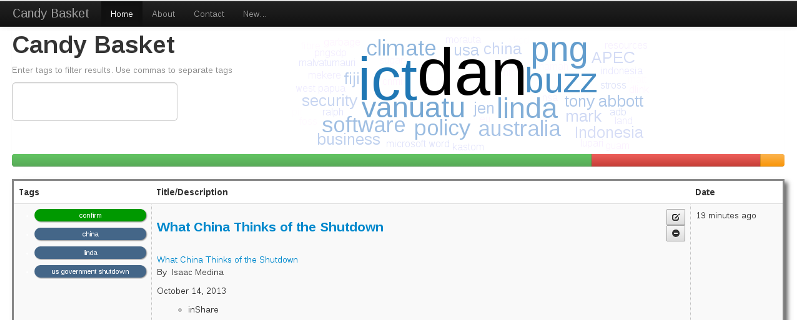
\includegraphics{candy-basket.png}\hfill}


\subsection{Logging in}
\label{user-guide:logging-in}
In order to access Mnemoniq you will need to begin by typing in the
address of the URL. A username and password will be requested: once
you have entered them you will be taken to the Home page, an example
of which is shown in the screenshot below. The interface is designed
to work with touch, allowing you to use a mobile platform for ease of
entry and constant availability. This also allows you to enter the
information in an unobtrusive fashion.


\subsection{Toolbar}
\label{user-guide:toolbar}
The black toolbar running along the top of the screen allows you to
navigate between pages and contains four options:
\begin{itemize}
\item {} 
\textbf{Home} The Home option takes you back to the main display page, such as the one displayed in the screenshot above.

\item {} 
\textbf{About} Contains links to the documentation.

\item {} 
\textbf{Contact} Contains contact information.

\item {} 
\textbf{Add new...} The Add new function allows you to add a new entry into the database.

\end{itemize}


\subsection{Header}
\label{user-guide:header}
The page contains a header and a subtitle at the top of the page,
below the toolbar, which you can define yourself.

{\hfill
\includegraphics{candy-basket-header.png}\hfill}


\subsection{Entry bar}
\label{user-guide:entry-bar}
The entry bar (or search bar) allows entries to be selected
according to their tags. By entering keywords in the entry bar only
those entries which have been tagged with those keywords will be
selected. You can enter two or more words into the entry bar,
separated by a space, and only those entries which have been tagged with
both words will be displayed. By clicking the \emph{X} on each tag you
will return to the full list of entries.

{\hfill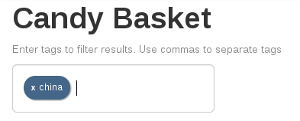
\includegraphics{candy-basket-search.png}\hfill}


\subsection{Word cloud}
\label{user-guide:word-cloud}
The word cloud displays all the tags which have been entered so
far. The size of the words reflects the number of times the tag has
been entered. The cloud is also clickable, giving you an
alternative way of selecting a group of entries. By clicking on one
of the words in the cloud, only those entries which have that tag will
be displayed.

{\hfill
\includegraphics{candy-basket-wordcloud.png}\hfill}

Once you have selected a tag, using either the entry bar or the word
cloud, the word cloud updates itself to reflect the tags in the refined
selection. You may then select a second tag by again clicking on the
word cloud. The previous search will not be cleared by doing so.


\subsection{Tagging}
\label{user-guide:tagging}
Tagging is the most important component of the software.


\subsection{General tags}
\label{user-guide:general-tags}
Once an entry has added, the tags associated with that entry will be
displayed on the left hand side. Tags are designed to be:
\begin{itemize}
\item {} 
Short

\item {} 
Immediately comprehensible

\item {} 
Lower case

\item {} 
Not categories, but flexible

\item {} 
Intuitive

\item {} 
Technical jargon may be useful, as shadowing the language which is spoken within the user group may facilitate precision.

\item {} 
As you begin to specify a tag for an entry, tags which have already been entered will come up as suggestions. There are two reasons for this function, which is not intended to be prescriptive. For practical reasons, as it facilitates ease of entry on a mobile device and, importantly, it allows the number of equivalent tags to be reduced to reduce in order to streamline functions such as the word cloud.

\end{itemize}

{\hfill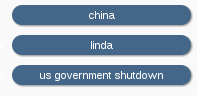
\includegraphics{candy-basket-generaltags.png}\hfill}


\subsection{Supertags}
\label{user-guide:supertags}
A supertag is a special type of tag which will be coloured in either
green, yellow or red according to its content. This is a structured
form of tagging. While the other tags provide context, supertags
classify the information according to whether or not the entry
confirms, surprises or challenges what you are currently doing and
thinking beliefs. These tags float to the top of the tag list, and the
bar across the top gives you a visual indication of the proportion of
super tags.  This is designed to show you how things appear to be
developing:
\begin{itemize}
\item {} 
if the entire line is green (Confirm) it would indicate that you are either being complacent or ignoring information that might suggest you should be doing things differently

\item {} 
if there is a high proportion of yellow, it could indicate you are working in a changing environment

\item {} 
if there is a high proportion of red, it may indicate two things. One interpretation could be that what you are doing is inappropriate.  Another interpretation is that what you are doing is generating a backlash—which you may in fact see as progress, particularly if you are trying to change the terms of a debate

\end{itemize}


\subsection{Tag count function}
\label{user-guide:tag-count-function}
The tag count function provides allows for a quick check-in of how
things appear to be going. However, should you be leaning heavily on
one category of supertag, you may want to think a little bit harder
about what the reason for that is. Given that employees are inputting
the information themselves, the information is easily biased in that
employees select which information is considered pertinent. Should you
find the majority of your supertags are:
\begin{itemize}
\item {} 
\textbf{Confirm}: then this would seem to indicate that you are being too complacent or ignoring challenging information (green).

\item {} 
\textbf{Surprise}: this may indicate, for example, a changing environment (yellow).

\item {} 
\textbf{Challenge}: this may suggest that the work being done by the organisation may be inappropriate or need revision (red).

\end{itemize}

{\hfill
\includegraphics{candy-basket-supertags-count.png}\hfill}

{\hfill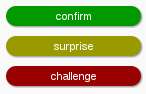
\includegraphics{candy-basket-supertags.png}\hfill}


\subsection{Add new entry}
\label{user-guide:add-new-entry}
When adding a new entry, there are four fields you need to fill in:
\begin{itemize}
\item {} 
The \emph{Source} entry bar allows you to specify the URL from which your information is sourced. Even if you enter information offline this field does need to be filled in, but you can enter anything such as a.com or offline.com

\item {} 
The \emph{Title} field allows you to specify a title for your entry

\item {} 
The \emph{Description} field should preferably be used to explain why you thought the entry was important.

\item {} 
The \emph{Tags} field is used to enter tags.

\end{itemize}

Once you have finished entering the fields select Save Changes and
Close to finish adding the entry. The entry then floats to the top of
the entry list, and the date it was created shows on the right hand
side.  If an entry is edited, the editing date is stored in the place
of the creation date, and it again floats to the top.

Submitting a new entry (or updating an existing one) will not be
accepted until the form is \emph{ready} for submission. For example, when
adding a new entry a form will look like this.

{\hfill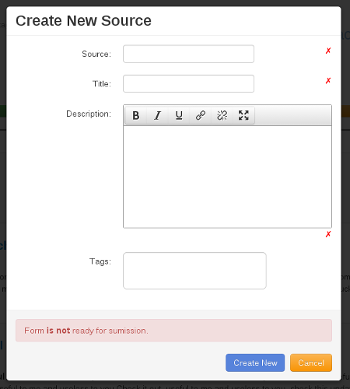
\includegraphics{candy-basket-add-not-ready.png}\hfill}

Once you start entering valid data the fields will be marked ready and
you will be able to submit your entry. It will be clear when the form
is ready for submission.

{\hfill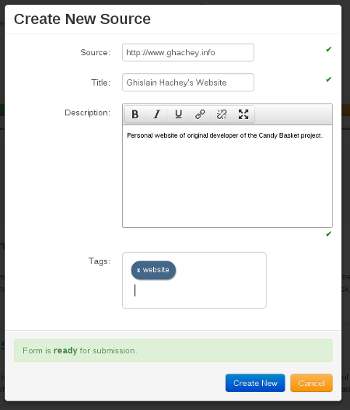
\includegraphics{candy-basket-add-ready.png}\hfill}


\subsection{Sources of information}
\label{user-guide:sources-of-information}
The information is added by individual employees. The tool is designed
to comprise external information, and may consist of anything, such
as:
\begin{itemize}
\item {} 
Photos

\item {} 
Web sites

\item {} 
Emails

\item {} 
Short pieces of text entered offline

\item {} 
Entering material which is not available online can either be manually

\end{itemize}

inputted, or the page number can be referenced. The URL can be
replaced with anything (such as offline.com), whether or not such an
URL exists.


\section{Contact details}
\label{user-guide:contact-details}
For more information, please contact:

\begin{tabulary}{\linewidth}{|L|L|L|L|L|}
\hline
\textsf{\relax 
Name
} & \textsf{\relax 
Organisation
} & \textsf{\relax 
Title
} & \textsf{\relax 
Issue
} & \textsf{\relax 
Email Address
}\\
\hline
Louise Shaxson
 & 
ODI
 & 
Research Fellow
 & 
Monitoring techniques, feedback and general support
 & 

\includegraphics{louise-email.png}
\\

Dan McGarry
 & 
PiPP
 & 
Chief technologist
 & 
Technical support
 & 

\includegraphics{dan-email.png}
\\

Derek Brien
 & 
PiPP
 & 
Executive Director and co-founder
 & 
Feedback
 & 

\includegraphics{derek-email.png}
\\
\hline\end{tabulary}



\chapter{Administrator Guide}
\label{administrator-guide:administrator-guide}\label{administrator-guide::doc}

\section{Introduction}
\label{administrator-guide:introduction}
\textbf{Note: Mnemoniq is referred herein as Candy Basket and memories and
candies for historical reasons. This will eventually be changed, but
for now the technical terminologies used are the old ones.}

This guide is meant for the person who wants to deploy Candy Basket in
its own environment. Candy Basket supports single signon for
authentication, and once authenticated users have full access to the
application. Candy Basket was tested to work with both Windows Server
2008 and Samba 4 as Active Directory and Domain Controller.

Candy Basket can be deployed on essentially any operating system using
any HTTP server. However, the only tested and supported approach is
deploying Candy Basket on the latest Debian 7 with Apache and WSGI.


\section{Pre-Built VMWare Image}
\label{administrator-guide:pre-built-vmware-image}
The supported way of deploying Candy Basket is the pre-built VMWare
image. This image comes ready to be deployed to your VMware
infrastructure with minimal configuration.

The installation of the image should be a simple matter of booting it
from your VMware host server. However, you will need to correctly
setup networking, preferably in bridge mode where it will live
side-by-side with the rest of the network. You will need to assign it
a static IP address.

It is assumed you run your own internal DNS. You will need to add your
chosen fully qualified host name as an A record to this new server,
for example:

\begin{Verbatim}[commandchars=\\\{\}]
192.168.1.10     A      candy.pacificpolicy.org
\end{Verbatim}

Reverse DNS must also be working for single sign-on to work. Once the
new server is part of your network and you can correctly ping it using
its host name you will need to change the domain name in several
places.
\begin{itemize}
\item {} 
All three Apache Virtual Hosts configuration in
\emph{/etc/apache2/sites-available/}

\item {} 
The CORS Python file in
\emph{/srv/www-apps/candybasket/backend/config.py}. The allowed domains
should be identified there. This should a single fully qualified
host name such as \emph{candy.pacificpolicy.org}.

\item {} 
The Candy Basket RESTful service location in
\emph{/srv/www-apps/candybasket/frontend/static/js/services.js}. The
variable \emph{wsUrl} should be changed to your own fully qualified host
name.

\end{itemize}

Restart Apache, tail -f its \emph{/var/log/error.log} file and try
pointing your browser to \emph{https://candy.pacificpolicy.org}.


\section{VMWare Test Environment}
\label{administrator-guide:vmware-test-environment}
If you are interested in improving the VMWare image or anything in the
build process these notes might come in handy to create your own test
environment. We use VMware workstation with a number of VMware Virtual
Machines (VM) to simulate a production environment. On my machines I
create the following VMs:
\begin{itemize}
\item {} \begin{description}
\item[{\textbf{debian.pacificpolicy.org} the machine running the Candy Basket}] \leavevmode
application deployed as detailed in {\hyperref[administrator-guide:deploy-debian-apache]{deploy-debian-apache}}

\end{description}

\item {} \begin{description}
\item[{\textbf{winserver2008.pacificpolicy.org} An Active Directory and Domain}] \leavevmode
Controller running Windows Server 2008

\end{description}

\item {} \begin{description}
\item[{\textbf{samba4.pacificpolicy.org} An Active Directory and Domain}] \leavevmode
Controller running Samba4 on Debian

\end{description}

\item {} 
\textbf{win7.pacificpolicy.org} A Windows 7 workstion

\end{itemize}


\subsection{VMWare Vitual Machines Lab Setup}
\label{administrator-guide:vmware-vitual-machines-lab-setup}\begin{itemize}
\item {} 
Install VMware workstation

\item {} 
Create a number of vitual machines: one Windows Server 2008
(winserver2008.pacificpolicy.org), one Windows 7 Pro
(win7.pacificpolicy.org), one Windows 8 Pro
(win8.pacificpolicy.org), one Debian Linux to host software
application (server.pacificpolicy.org).

\item {} 
Create a private LAN Segment. This can be done in any VM's LAN
settings.

\item {} 
Configure the Windows server 2008 VM with two virtual network
interfaces: one will NAT from the host and the other should be part
of a the private LAN segment.

\item {} 
Configure the VMs that will be part of the domain (Win7, Win8 and
Debian Linux) with the private LAN segment for networking.

\end{itemize}


\subsection{Windows Server 2008 Configuration}
\label{administrator-guide:windows-server-2008-configuration}
Open the Server Manager and add and configure necessary roles including:
\begin{itemize}
\item {} 
Active Directory Domain Services steps.

\item {} 
DHCP Server (e.g. assign a pool of 192.168.30.100-200 on the Windows
server internal network interfaces with static IP of 192.168.30.1)

\item {} 
DNS Server (e.g. create A records for all machines in the test lab:
win7.pacificpolicy.org, debian.pacificpolicy.org,
winserver2008.pacificpolicy.org and add CNAME records for services
on the debian server, something like CNAME www.pacificpolicy.org -\textgreater{}
debian.pacificpolicy.org)

\item {} 
Network Policy and Access Services (to turn it into a Gateway
(Route/NAT)) step.

\end{itemize}

If you want to access private VMs using SSH from your host you could
port forward traffic through the Windows Server with the following
commands:

\begin{Verbatim}[commandchars=\\\{\}]
C:\PYGZbs{}\PYGZgt{} netsh interface portproxy add v4tov4 listenport=2222 listenaddress=172.16.228.136 connectport=22 connectaddress=192.168.20.10
\end{Verbatim}


\subsection{Join Domain with Windows VMs}
\label{administrator-guide:join-domain-with-windows-vms}
Boot the VMs and verify that networking is working correctly. Make
sure IP addresses are assigned according to the DHCP pool configure in
the previous step. Test DNS with nslookup or simple ping:

\begin{Verbatim}[commandchars=\\\{\}]
[root]\PYGZdl{} nslookup winserver2008.pacificpolicy.org
[root]\PYGZdl{} nslookup win7.pacificpolicy.org
[root]\PYGZdl{} nslookup server.pacificpolicy.org
\end{Verbatim}

If the Windows Server was correctly setup as a gateway in ``Network
Policy and Access Services'' access to the Internet should work. Verify
that the time is correctly being synced with Internet servers. You
should now be able to join the domain.


\subsection{Join Domain with the Linux Server VM}
\label{administrator-guide:join-domain-with-the-linux-server-vm}
The Linux server can make use of a static IP address. The appropriate
A record should be added to the Windows Server 2008 DNS zone
file. Test networking (DNS and Internet access) and join the domain as
a samba client.

Regarding Linux Guest VMs, VMWare specifically recommends to use NTP
on the guest instead of the VMware's time syncing feature (see
here). Since time sync is critical for the proper functioning of the
single signon authentication it is better to be safe and follow best
practices.  Installing ntp on Debian is easy:

\begin{Verbatim}[commandchars=\\\{\}]
[root]\PYGZdl{} aptitude install ntp
\end{Verbatim}

The default values in /etc/ntp.conf are fine, but it is recommended by
VMware to add the following line to make sure ntp always syncs
regarless of any large time jump it observes between Internet NTP
servers and local OS time:

\begin{Verbatim}[commandchars=\\\{\}]
tinker panic 0
\end{Verbatim}

then restart ntp:

\begin{Verbatim}[commandchars=\\\{\}]
[root]\PYGZdl{} service ntp restart
\end{Verbatim}

You might find it useful to allow yourself to SSH inside the Debian
VMware from your host terminal; otherwise, getting in and out of the
VM's terminal is annoying and you loose the ability to copy/paste from
host to VM. Apparently setting up port forwarding on Windows Server
2008 R2 through the GUI is cmpletely broken. I have not tested this
myself, but it is easy to do on the command line as detailed here.


\section{Deployment on Debian with Apache HTTP server}
\label{administrator-guide:deployment-on-debian-with-apache-http-server}\label{administrator-guide:deploy-debian-apache}
The steps to deploy Candy Basket on a production Debian server are
very similar to setting up Candy Basket in a development environment.


\subsection{Oerating System}
\label{administrator-guide:oerating-system}
Download an ISO of the latest Debian and do a bare installation with
only the standard utilities and SSH. You may also install any other
useful packages you will most likely eventually need such as rsync,
ntp, curl, wget.

\begin{Verbatim}[commandchars=\\\{\}]
[root]\PYGZdl{} aptitude install rsync ntp sudo curl wget vim locate screen zip git
\end{Verbatim}

Create a user to `own' the Candy Basket application

\begin{Verbatim}[commandchars=\\\{\}]
[root]\PYGZdl{} adduser candy
\end{Verbatim}


\subsection{Dependencies}
\label{administrator-guide:dependencies}
Install the Apache HTTP server with Python support.

\begin{Verbatim}[commandchars=\\\{\}]
[root]\PYGZdl{} aptitude install apache2 libapache2\PYGZhy{}mod\PYGZhy{}wsgi python\PYGZhy{}dev
\end{Verbatim}

Install Python and preferably virtualenv to cleanly isolate the
application and its dependencies. This process is exactly as defined
in {\color{red}\bfseries{}python-and-virtualenv\_}. The only difference in production
will be the creation of an BASELINE virtual environment for Apache:
this is an empty virtual environment with its own clean Python
installation meant to power Python web applications. The BASELINE
virtual environment could be owned by any user but in this case we
will make use of the \emph{candy} user.

Create the BASELINE.

\begin{Verbatim}[commandchars=\\\{\}]
[candy]\PYGZdl{} mkvirtualenv BASELINE
\end{Verbatim}

And finally, tell Apache about it by adding the following line in
\emph{/etc/apache2/conf.d/wsgi.conf}.

\begin{Verbatim}[commandchars=\\\{\}]
WSGIPythonHome  /home/candy/.virtualenvs/BASELINE
\end{Verbatim}

At this point, you should have two virgin virtual environments, test
it before going further.

\begin{Verbatim}[commandchars=\\\{\}]
[candy]\PYGZdl{} lsvirtualenv
BASELINE
========

candy.pacificpolicy.org
=======================
\end{Verbatim}

Install CouchDB in a similar way as you would in a development
environment. In production, CouchDB can also be owned by \emph{candy}
instead of \emph{root}. The new Linux Filesystem Hierarchy Standard {\hyperref[developer-guide:fhs]{{[}FHS{]}}}
recommends installing such ``non-distro provided'' or optional software
in \emph{/opt/}. As user \emph{root}, make a nice place for it.

\begin{Verbatim}[commandchars=\\\{\}]
[root]\PYGZdl{} mkdir /opt/candy/
[root]\PYGZdl{} chown candy:candy \PYGZhy{}R /opt/candy/
\end{Verbatim}

As user \emph{candy}, install CouchDB as detailed in
{\color{red}\bfseries{}couchdb\_}. Couchdb dependencies will have to be installed as
\emph{root}, of course. In production it would be a good idea to have an
init script. On Debian you can simply edit the distribution provided
\emph{/etc/init.d/skeleton}. Test you correctly created the init script:

\begin{Verbatim}[commandchars=\\\{\}]
[root]\PYGZdl{} /etc/init.d/couchdb start
[root]\PYGZdl{} ps \PYGZhy{}ef \textbar{} grep couch
(couchdb processes running)
[root]\PYGZdl{} /etc/init.d/couchdb stop
[root]\PYGZdl{} ps \PYGZhy{}ef \textbar{} grep couch
(no couchdb process output)
[root]\PYGZdl{} /etc/init.d/couchdb restart
\end{Verbatim}

Once the init script is working you can instruct the system to start
it on boot:

\begin{Verbatim}[commandchars=\\\{\}]
[root]\PYGZdl{} update\PYGZhy{}rc.d couchdb default
\end{Verbatim}

You should not be able to login CouchDB by pointing your browser to
\emph{http://localhost:5984/\_utils} or \emph{http://ip.address:5984/\_utils} if
you are connecting from a remote machine although by default CouchDB
listens on localhost so this would involved changing the
configuration.  From the administrative interface create a database
with the name \emph{candybasketng} and add the design documents
(i.e. views) located in \emph{db/views/docs/}.


\subsection{Candy Basket as Apache Virtual Host}
\label{administrator-guide:candy-basket-as-apache-virtual-host}
The final step to deploy the Candy Basket application. Create a
directory where the application will be served from:

\begin{Verbatim}[commandchars=\\\{\}]
[root]\PYGZdl{} mkdir \PYGZhy{}p /srv/www\PYGZhy{}apps/candybasket/
\end{Verbatim}

More work will be done to improve the development to production
workflow cycle but for now simply \emph{rsync} the whole source tree into
\emph{/srv/www-apps/candy.pacificpolicy.org/}. Let's assume you have the
latest source checked out in \emph{/home/candy/}:

\begin{Verbatim}[commandchars=\\\{\}]
[root]\PYGZdl{} rsync \PYGZhy{}avg /home/candy/tagging\PYGZhy{}tool/ /srv/www\PYGZhy{}apps/candybasket/
[root]\PYGZdl{} chown candy:www\PYGZhy{}data \PYGZhy{}R /srv/www\PYGZhy{}apps/candybasket/
\end{Verbatim}

Create three Apache virtual hosts: one for the Candy Basket REST
service and two for the Candy Basket application (HTTP and
HTTPS). Sample configuration are included below.

\emph{candybasket.http}:

\begin{Verbatim}[commandchars=\\\{\}]
\PYGZlt{}VirtualHost *:80\PYGZgt{}
        ServerName candy.pacificpolicy.org
        ServerAlias candy candy.pacificpolicy.org.vu
        ServerAdmin admin@localhost

        RewriteEngine on
        ReWriteCond \PYGZpc{}\PYGZob{}SERVER\PYGZus{}PORT\PYGZcb{} !\PYGZca{}443\PYGZdl{}
        RewriteRule \PYGZca{}/(.*) https://\PYGZpc{}\PYGZob{}HTTP\PYGZus{}HOST\PYGZcb{}/\PYGZdl{}1 [NC,R,L]

        ErrorLog \PYGZdl{}\PYGZob{}APACHE\PYGZus{}LOG\PYGZus{}DIR\PYGZcb{}/error.log
        LogLevel warn
        CustomLog \PYGZdl{}\PYGZob{}APACHE\PYGZus{}LOG\PYGZus{}DIR\PYGZcb{}/access.log combined
\PYGZlt{}/VirtualHost\PYGZgt{}
\end{Verbatim}

\emph{candybasket.https}:

\begin{Verbatim}[commandchars=\\\{\}]
\PYGZlt{}IfModule mod\PYGZus{}ssl.c\PYGZgt{}
\PYGZlt{}VirtualHost *:443\PYGZgt{}
        ServerName candy.pacificpolicy.org.vu
        ServerAlias candy candy.pacificpolicy.org
        ServerAdmin admin@localhost

        DocumentRoot /srv/www\PYGZhy{}apps/candybasket/frontend/

        \PYGZlt{}Directory /srv/www\PYGZhy{}apps/candybasket/frontend/\PYGZgt{}
                Order allow,deny
                Allow from all
        \PYGZlt{}/Directory\PYGZgt{}

        Alias /help /srv/www\PYGZhy{}apps/candybasket/docs/build/html/

        ProxyPass /basket http://candy\PYGZhy{}restapi\PYGZhy{}v1.pacificpolicy.org.vu/basket
        ProxyPassReverse /basket http://candy\PYGZhy{}restapi\PYGZhy{}v1.pacificpolicy.org.vu/basket

        ErrorLog \PYGZdl{}\PYGZob{}APACHE\PYGZus{}LOG\PYGZus{}DIR\PYGZcb{}/error.log
        LogLevel warn
        CustomLog \PYGZdl{}\PYGZob{}APACHE\PYGZus{}LOG\PYGZus{}DIR\PYGZcb{}/ssl\PYGZus{}access.log combined

        SSLEngine on
        SSLCertificateFile    /etc/ssl/certs/ssl\PYGZhy{}cert\PYGZhy{}snakeoil.pem
        SSLCertificateKeyFile /etc/ssl/private/ssl\PYGZhy{}cert\PYGZhy{}snakeoil.key

        \PYGZlt{}FilesMatch \PYGZdq{}\PYGZbs{}.(cgi\textbar{}shtml\textbar{}phtml\textbar{}php)\PYGZdl{}\PYGZdq{}\PYGZgt{}
                SSLOptions +StdEnvVars
        \PYGZlt{}/FilesMatch\PYGZgt{}

        \PYGZlt{}Directory /usr/lib/cgi\PYGZhy{}bin\PYGZgt{}
                SSLOptions +StdEnvVars
        \PYGZlt{}/Directory\PYGZgt{}

        BrowserMatch \PYGZdq{}MSIE [2\PYGZhy{}6]\PYGZdq{} \PYGZbs{}
                nokeepalive ssl\PYGZhy{}unclean\PYGZhy{}shutdown \PYGZbs{}
                downgrade\PYGZhy{}1.0 force\PYGZhy{}response\PYGZhy{}1.0
        \PYGZsh{} MSIE 7 and newer should be able to use keepalive
        BrowserMatch \PYGZdq{}MSIE [17\PYGZhy{}9]\PYGZdq{} ssl\PYGZhy{}unclean\PYGZhy{}shutdown
\PYGZlt{}/VirtualHost\PYGZgt{}
\PYGZlt{}/IfModule\PYGZgt{}
\end{Verbatim}

\emph{candybasket-restapi-v1}:

\begin{Verbatim}[commandchars=\\\{\}]
\PYGZlt{}VirtualHost *:80\PYGZgt{}
        ServerName candy\PYGZhy{}restapi\PYGZhy{}v1.pacificpolicy.org
        ServerAlias candy\PYGZhy{}restapi\PYGZhy{}v1 candy\PYGZhy{}restapi\PYGZhy{}v1.pacificpolicy.org.vu
        ServerAdmin admin@localhost

        WSGIDaemonProcess runservice user=www\PYGZhy{}data group=www\PYGZhy{}data processes=1 threads=5
        WSGIScriptAlias / /srv/www\PYGZhy{}apps/candybasket/backend/runservice.wsgi

        \PYGZlt{}Directory /srv/www\PYGZhy{}apps/candybasket/backend/\PYGZgt{}
\PYGZsh{}               Header set Access\PYGZhy{}Control\PYGZhy{}Allow\PYGZhy{}Origin \PYGZdq{}*\PYGZdq{}
\PYGZsh{}               Header set Access\PYGZhy{}Control\PYGZhy{}Allow\PYGZhy{}Credentials true
                WSGIProcessGroup runservice
                WSGIApplicationGroup \PYGZpc{}\PYGZob{}GLOBAL\PYGZcb{}
                WSGIScriptReloading On
                Order deny,allow
                Allow from all
        \PYGZlt{}/Directory\PYGZgt{}

        ErrorLog \PYGZdl{}\PYGZob{}APACHE\PYGZus{}LOG\PYGZus{}DIR\PYGZcb{}/error.log
        LogLevel warn
        CustomLog \PYGZdl{}\PYGZob{}APACHE\PYGZus{}LOG\PYGZus{}DIR\PYGZcb{}/access.log combined
\PYGZlt{}/VirtualHost\PYGZgt{}
\end{Verbatim}

Enable the needed modules and the new virtual hosts and then restart Apache:

\begin{Verbatim}[commandchars=\\\{\}]
[root]\PYGZdl{} a2ensite candybasket.http
[root]\PYGZdl{} a2ensite candybasket.https
[root]\PYGZdl{} a2ensite candybasket\PYGZhy{}restapi\PYGZhy{}v1
[root]\PYGZdl{} a2enmod ssl
[root]\PYGZdl{} a2enmod rewrite
[root]\PYGZdl{} a2enmod proxy
[root]\PYGZdl{} a2enmod proxy\PYGZus{}http

[root]\PYGZdl{} service apache2 restart
\end{Verbatim}

Make sure name resolution is working for the domains used in the
Apache Virtual Hosts. If you you do not have internal DNS adding the
records in the servers' \emph{/etc/hosts} file will work:

\begin{Verbatim}[commandchars=\\\{\}]
127.0.0.1       candy.pacificpolicy.org
127.0.0.1       candy\PYGZhy{}restapi\PYGZhy{}v1.pacificpolicy.org
127.0.0.1       candy.pacificpolicy.org.vu
127.0.0.1       candy\PYGZhy{}restapi\PYGZhy{}v1.pacificpolicy.org.vu
\end{Verbatim}

Connect to the \emph{candy} virtualenv and install Candy Basket's Python
dependencies:

\begin{Verbatim}[commandchars=\\\{\}]
[candy]\PYGZdl{} workon candy.pacificpolicy.org
(candy.pacificpolicy.org)[candy]\PYGZdl{} cd /srv/www\PYGZhy{}apps/candybasket/backend/
(candy.pacificpolicy.org)[candy]\PYGZdl{} pip install \PYGZhy{}r requirements.pip
\end{Verbatim}

As a final step to make sure that all the bits connect together the
WSGI script \emph{/srv/www-apps/candybasket/backend/runservice.wsgi} should
be verified. It is mostly also preconfigured except that the following
two lines will depend on your own environment: what did you call the
Python virtualenv (it's \emph{candy} here) and what Python version is
running on your OS. If steps herein were closely followed the
following two lines should be edited and uncommented to look like:

\begin{Verbatim}[commandchars=\\\{\}]
\PYG{c}{\PYGZsh{} If using virtualenv, add the virtualenv\PYGZsq{}s site\PYGZhy{}packages to sys.path as well}
\PYG{n}{VENV\PYGZus{}PATH} \PYG{o}{=} \PYG{l+s}{\PYGZdq{}}\PYG{l+s}{/home/candy/.virtualenvs/candy.pacificpolicy.org/}\PYG{l+s}{\PYGZdq{}}
\PYG{n}{site}\PYG{o}{.}\PYG{n}{addsitedir}\PYG{p}{(}\PYG{n}{os}\PYG{o}{.}\PYG{n}{path}\PYG{o}{.}\PYG{n}{join}\PYG{p}{(}\PYG{n}{VENV\PYGZus{}PATH}\PYG{p}{,}\PYG{l+s}{\PYGZsq{}}\PYG{l+s}{lib/python2.7/site\PYGZhy{}packages/}\PYG{l+s}{\PYGZsq{}}\PYG{p}{)}\PYG{p}{)}
\end{Verbatim}

Restart Apache, tail -f its \emph{/var/log/error.log} file and try pointing
your browser to \emph{https://candy.pacificpolicy.org}. At this point you
should have a fully working albeit insecured installation of Candy
Basket.


\section{Windows Active Directory and Apache Kerberos Single Sign-on}
\label{administrator-guide:windows-active-directory-and-apache-kerberos-single-sign-on}
Candy Basket can be securely deployed in a Windows environment with
users authenticating to it using single signon (SOO). In other words,
members of the domain that are logged in the network should be able to
access the web application securely without providing credentials.


\subsection{Install Necessary Software}
\label{administrator-guide:install-necessary-software}
Some kerberos, Apache and samba packages are needed:

\begin{Verbatim}[commandchars=\\\{\}]
[root]\PYGZdl{} aptitude install apache2\PYGZhy{}mpm\PYGZhy{}prefork libapache2\PYGZhy{}mod\PYGZhy{}auth\PYGZhy{}kerb
[root]\PYGZdl{} aptitude install krb5\PYGZhy{}config krb5\PYGZhy{}user krb5\PYGZhy{}clients samba\PYGZhy{}client ntp
\end{Verbatim}


\subsection{Time Synchronization}
\label{administrator-guide:time-synchronization}
This setup is high sensitive to clocks being in sync. The network time
protocol is the best approach to make things work:

\begin{Verbatim}[commandchars=\\\{\}]
[root]\PYGZdl{} aptitude install ntp
\end{Verbatim}

The default values in \emph{/etc/ntp.conf} are fine. However, ntp will stop
syncing if it detects a large enough jump in time as it assumes you
are getting time from an invalid source.  Syncing using the provided
default OS' ntp servers should be safe. If you are on VMware or
anywhere the time may drift easily it would be a good idea to always
sync regarless of any large time jump; it can be achieved by adding
the following line at the top of \emph{/etc/ntp.conf}:

\begin{Verbatim}[commandchars=\\\{\}]
tinker panic 0
\end{Verbatim}

then restart ntp:

\begin{Verbatim}[commandchars=\\\{\}]
[root]\PYGZdl{} service ntp restart
\end{Verbatim}


\subsection{DNS Configuration}
\label{administrator-guide:dns-configuration}
The setup here as three machines: a Windows Server 2008 RC2 with
Active Directory and Domain Controller, a Debian werver running the
web service and a Windows 7 workstation. Forward and reverse DNS
should be configured something like this:

\begin{Verbatim}[commandchars=\\\{\}]
winserver2008.pacificpolicy.org    A    192.168.30.1
debian.pacificpolicy.org    A    192.168.30.10
www.pacificpolicy.org    CNAME    debian.pacificpolicy.org
test.pacificpolicy.org    CNAME    debian.pacificpolicy.org
\end{Verbatim}

Make sure everything resolves as it should from within
win7.pacificpolicy.org:

\begin{Verbatim}[commandchars=\\\{\}]
[root]\PYGZdl{} nslookup debian.pacificpolicy.org
Server:        192.168.30.1
Address:    192.168.30.1\PYGZsh{}53
Name:    debian.pacificpolicy.org
Address: 192.168.30.10

[root]\PYGZdl{} nslookup www.pacificpolicy.org
Server:        192.168.30.1
Address:    192.168.30.1\PYGZsh{}53
www.pacificpolicy.org    canonical name = debian.pacificpolicy.org.
Name:    www.pacificpolicy.org
Address: 192.168.30.10

[root]\PYGZdl{} nslookup 192.168.30.10
Server:        192.168.30.1
Address:    192.168.30.1\PYGZsh{}53
10.30.168.192.in\PYGZhy{}addr.arpa    name = debian.pacificpolicy.org.
\end{Verbatim}


\subsection{Kerberos configuration}
\label{administrator-guide:kerberos-configuration}
Back on the Debian server, backup the original and create your own:

\begin{Verbatim}[commandchars=\\\{\}]
[root]\PYGZdl{} sudo cp /etc/krb5.conf /etc/krb5.conf.bak

[libdefaults]
        default\PYGZus{}realm = PACIFICPOLICY.ORG
        \PYGZsh{} The following krb5.conf variables are only for MIT Kerberos.
        krb4\PYGZus{}config = /etc/krb.conf
        krb4\PYGZus{}realms = /etc/krb.realms
        kdc\PYGZus{}timesync = 1
        ccache\PYGZus{}type = 4
        forwardable = true
        proxiable = true

[realms]
        PACIFICPOLICY.ORG = \PYGZob{}
                kdc = winserver2008.pacificpolicy.org
                master\PYGZus{}kdc = winserver2008.pacificpolicy.org
                admin\PYGZus{}server = winserver2008.pacificpolicy.org
                default\PYGZus{}domain = pacificpolicy.org
        \PYGZcb{}

[domain\PYGZus{}realm]
        .pacificpolicy.org = PACIFICPOLICY.ORG
        pacificpolicy.org = PACIFICPOLICY.ORG

[login]
        krb4\PYGZus{}convert = true
        krb4\PYGZus{}get\PYGZus{}tickets = false
\end{Verbatim}

Test Kerberos by getting a ticket-granting ticket (TGT) for the domain
controller's Administrator user:

\begin{Verbatim}[commandchars=\\\{\}]
[root]\PYGZdl{} kinit Administrator
Password for Administrator@PACIFICPOLICY.ORG:
[root]\PYGZdl{} klist
Ticket cache: FILE:/tmp/krb5cc\PYGZus{}0
Default principal: Administrator@PACIFICPOLICY.ORG

Valid starting    Expires           Service principal
24/10/2013 15:13  25/10/2013 01:13  krbtgt/PACIFICPOLICY.ORG@PACIFICPOLICY.ORG
    renew until 25/10/2013 15:13
\end{Verbatim}


\subsection{Configure Samba to Join the Domain}
\label{administrator-guide:configure-samba-to-join-the-domain}
Backup the original configuration and use the minimal configuration below:

\begin{Verbatim}[commandchars=\\\{\}]
[root]\PYGZdl{} cp /etc/samba/smb.conf /etc/samba/smb.conf.bak

[global]
        netbios name = debian
        realm = PACIFICPOLICY.ORG
        workgroup = PACIFICPOLICY
        server string = \PYGZpc{}h server
        dns proxy = no
        log file = /var/log/samba/log.\PYGZpc{}m
        max log size = 1000
        panic action = /usr/share/samba/panic\PYGZhy{}action \PYGZpc{}d
        security = ADS
        password server = winserver2008.pacificpolicy.org
        encrypt passwords = true
        passdb backend = tdbsam
        obey pam restrictions = yes
        unix password sync = yes
        passwd program = /usr/bin/passwd \PYGZpc{}u
        passwd chat = *Enter\PYGZbs{}snew\PYGZbs{}s*\PYGZbs{}spassword:* \PYGZpc{}n\PYGZbs{}n *Retype\PYGZbs{}snew\PYGZbs{}s*\PYGZbs{}spassword:* \PYGZpc{}n\PYGZbs{}n *password\PYGZbs{}supdated\PYGZbs{}ssuccessfully* .
        pam password change = yes
        map to guest = bad user
        kerberos method = dedicated keytab
\end{Verbatim}


\subsection{Join the domain}
\label{administrator-guide:join-the-domain}
The server should be a member of the domain; this is easy with Samba:

\begin{Verbatim}[commandchars=\\\{\}]
[root]\PYGZdl{} net ads join \PYGZhy{}U Administrator
Enter Administrator\PYGZsq{}s password:
Using short pacificpolicy.org \PYGZhy{}\PYGZhy{} PACIFICPOLICY
Joined \PYGZsq{}SERVER\PYGZsq{} to realm \PYGZsq{}pacificpolicy.org\PYGZsq{}
\end{Verbatim}

If the domain is joined successfully a new Active Directory account
will be created. That machine account could be used but I opted to
create a specific user to handle authentication of the service. On the
windows server add a new AD user account (e.g. I add a user HTTP
Service with user httpservice) and make sure the password can not be
reset and will last foreever.

Now you need to create the `principle': someone or something to
authenticate or authenticate to (e.g. users, services). This can be a
little tricky and there are a few ways to achieve this. Use the kpass
utility to create the keytab with the principal; it will both add the
service principal to the user and create a keytab which can later be
used by a service such as Apache:

\begin{Verbatim}[commandchars=\\\{\}]
C:\PYGZbs{}\PYGZgt{} ktpass \PYGZhy{}princ HTTP/debian.pacificpolicy.org@PACIFICPOLICY.ORG
\PYGZhy{}mapuser httpservice@PACIFICPOLICY.ORG
\PYGZhy{}crypto RC4\PYGZhy{}HMAC\PYGZhy{}NT
\PYGZhy{}ptype KRB5\PYGZus{}NT\PYGZus{}PRINCIPAL
\PYGZhy{}pass somepassword
\PYGZhy{}out c:\PYGZbs{}Temp\PYGZbs{}krb5.keytab
\end{Verbatim}

Copy the file \emph{c:\textbackslash{}Temp\textbackslash{}krb5.keytab} on the Debian server somewhere
appropriate (e.g. \emph{/etc/krb5.keytab}). Assign correct ownership and
permissions:

\begin{Verbatim}[commandchars=\\\{\}]
[root]\PYGZdl{} chown root.www\PYGZhy{}data /etc/krb5.keytab
[root]\PYGZdl{} chmod 0640 /etc/krb5.keytab
\end{Verbatim}

This should be it, but some testing will help. Get a Ticket-Granting
Ticket (TGT) for the service principal:

\begin{Verbatim}[commandchars=\\\{\}]
[root]\PYGZdl{} kinit HTTP/debian.pacificpolicy.org@PACIFICPOLICY.ORG
\end{Verbatim}

View the ticket from the cache:

\begin{Verbatim}[commandchars=\\\{\}]
[root]\PYGZdl{} klist
Ticket cache: FILE:/tmp/krb5cc\PYGZus{}0
Default principal: HTTP/debian.pacificpolicy.org@PACIFICPOLICY.ORG

Valid starting    Expires           Service principal
30/10/2013 16:20  31/10/2013 02:20  krbtgt/PACIFICPOLICY.ORG@PACIFICPOLICY.ORG
    renew until 31/10/2013 16:20
\end{Verbatim}

Get a service ticket for the principal:

\begin{Verbatim}[commandchars=\\\{\}]
[root]\PYGZdl{} kvno HTTP/debian.pacificpolicy.org@PACIFICPOLICY.ORG
HTTP/debian.pacificpolicy.org@PACIFICPOLICY.ORG: kvno = 4
\end{Verbatim}

List what is in the ticket cache and make sure you show the encryption
type usig the `-e' flag:

\begin{Verbatim}[commandchars=\\\{\}]
[root]\PYGZdl{} klist \PYGZhy{}e
Ticket cache: FILE:/tmp/krb5cc\PYGZus{}0
Default principal: HTTP/debian.pacificpolicy.org@PACIFICPOLICY.ORG

Valid starting    Expires           Service principal
30/10/2013 16:20  31/10/2013 02:20  krbtgt/PACIFICPOLICY.ORG@PACIFICPOLICY.ORG
    renew until 31/10/2013 16:20, Etype (skey, tkt): aes256\PYGZhy{}cts\PYGZhy{}hmac\PYGZhy{}sha1\PYGZhy{}96, aes256\PYGZhy{}cts\PYGZhy{}hmac\PYGZhy{}sha1\PYGZhy{}96
30/10/2013 16:22  31/10/2013 02:20  HTTP/debian.pacificpolicy.org@PACIFICPOLICY.ORG
    renew until 31/10/2013 16:20, Etype (skey, tkt): arcfour\PYGZhy{}hmac, arcfour\PYGZhy{}hmac
\end{Verbatim}

Compare the service principal ticket above with the one from the
keytab file which will be used by Apache:

\begin{Verbatim}[commandchars=\\\{\}]
[root]\PYGZdl{} klist \PYGZhy{}e \PYGZhy{}k \PYGZhy{}t /etc/krb5.keytab
Keytab name: FILE:/etc/krb5.keytab
KVNO Timestamp        Principal
\PYGZhy{}\PYGZhy{}\PYGZhy{}\PYGZhy{} \PYGZhy{}\PYGZhy{}\PYGZhy{}\PYGZhy{}\PYGZhy{}\PYGZhy{}\PYGZhy{}\PYGZhy{}\PYGZhy{}\PYGZhy{}\PYGZhy{}\PYGZhy{}\PYGZhy{}\PYGZhy{}\PYGZhy{}\PYGZhy{} \PYGZhy{}\PYGZhy{}\PYGZhy{}\PYGZhy{}\PYGZhy{}\PYGZhy{}\PYGZhy{}\PYGZhy{}\PYGZhy{}\PYGZhy{}\PYGZhy{}\PYGZhy{}\PYGZhy{}\PYGZhy{}\PYGZhy{}\PYGZhy{}\PYGZhy{}\PYGZhy{}\PYGZhy{}\PYGZhy{}\PYGZhy{}\PYGZhy{}\PYGZhy{}\PYGZhy{}\PYGZhy{}\PYGZhy{}\PYGZhy{}\PYGZhy{}\PYGZhy{}\PYGZhy{}\PYGZhy{}\PYGZhy{}\PYGZhy{}\PYGZhy{}\PYGZhy{}\PYGZhy{}\PYGZhy{}\PYGZhy{}\PYGZhy{}\PYGZhy{}\PYGZhy{}\PYGZhy{}\PYGZhy{}\PYGZhy{}\PYGZhy{}\PYGZhy{}\PYGZhy{}\PYGZhy{}\PYGZhy{}\PYGZhy{}\PYGZhy{}\PYGZhy{}\PYGZhy{}\PYGZhy{}\PYGZhy{}\PYGZhy{}\PYGZhy{}
   4 01/01/1970 11:00 HTTP/debian.pacificpolicy.org@PACIFICPOLICY.ORG (arcfour\PYGZhy{}hmac)
\end{Verbatim}

The KVNO (password version number) , the encryption type and the
service principal name (i.e. \href{mailto:HTTP/debian.pacificpolicy.org@PACIFICPOLICY.ORG}{HTTP/debian.pacificpolicy.org@PACIFICPOLICY.ORG}) must
all match.  Apache VirtualHost Configuration

Add appropriate lines in the virtualhost to enable kerberos
authentication:

\begin{Verbatim}[commandchars=\\\{\}]
\PYGZlt{}VirtualHost *:80\PYGZgt{}
        ServerAdmin webmaster@localhost
        ServerName test.pacificpolicy.org

        DocumentRoot /srv/www\PYGZhy{}apps/test\PYGZhy{}single\PYGZhy{}signon

        \PYGZlt{}Directory /srv/www\PYGZhy{}apps/test\PYGZhy{}single\PYGZhy{}signon\PYGZgt{}
                Options Indexes FollowSymLinks MultiViews
                AllowOverride None
                Order allow,deny
                allow from all

                \PYGZsh{} Kerberos Single Signon
                AuthType Kerberos
                AuthName \PYGZdq{}Kerberos Login\PYGZdq{}
                KrbAuthRealms PACIFICPOLICY.ORG
                KrbServiceName HTTP
                KrbMethodNegotiate On
                KrbMethodK5Passwd On
                Krb5KeyTab /etc/krb5.keytab
                Require valid\PYGZhy{}user

        \PYGZlt{}/Directory\PYGZgt{}

        ErrorLog \PYGZdl{}\PYGZob{}APACHE\PYGZus{}LOG\PYGZus{}DIR\PYGZcb{}/error.log

        \PYGZsh{} Possible values include: debug, info, notice, warn, error, crit,
        \PYGZsh{} alert, emerg.
        LogLevel debug

        CustomLog \PYGZdl{}\PYGZob{}APACHE\PYGZus{}LOG\PYGZus{}DIR\PYGZcb{}/access.log combined
\PYGZlt{}/VirtualHost\PYGZgt{}
\end{Verbatim}


\subsection{Test from Client Workstations}
\label{administrator-guide:test-from-client-workstations}
Try login from a workstation that is joined to the domain and logged
in with a user; you should automatically be authenticated. You migvht
have to indicate to the Internet Explorer that the site you are
accessing is part of the Intranet. For example, add
\emph{http://*.pacificpolicy.org} to Internet \emph{Options-\textgreater{}Security-\textgreater{}Intranet-\textgreater{}Sites}.

Try with another workstion not joined to the domain; you should be
prompt to enter credentials.


\chapter{Developer Guide}
\label{developer-guide::doc}\label{developer-guide:developer-guide}

\section{Introduction}
\label{developer-guide:introduction}\label{developer-guide:intro}
This guide documents high level development standards, policies and
procedures without going into lower level details of the source code
and APIs.


\subsection{Programming Language}
\label{developer-guide:prog-lang}\label{developer-guide:programming-language}
The chosen programming language is Javascript both on the backend and
the frontend. Javascript is relatively easy to get started with, it is
increasingly popular to develop web applications and has a growing
wealth of libraries to use to build systems faster. \href{http://www.nodejs.org/}{NodeJS} is the Javascript backend platform and a
decent starting point and reference for the Javascript language is
provided by the \href{https://developer.mozilla.org/en-US/docs/Web/JavaScript}{Mozilla Developer Network}.


\subsection{Web Stack}
\label{developer-guide:web-stack}
No web application is built without a web framework (or library). The
prototype was built using Bottle/Flask in Python but the production
system will move to NodeJS and \href{http://expressjs.com/}{ExpressJS}. Both are good choices but moving to the
NodeJS has a number of advanges which were important to us including
pervasive use of asynchronous programming on backend and frontend
making it easier to scale with same amount of resources. A road to
unify backend and frontend languages, libraries and devleopment
tooling.

A micro framework was prefered to a full blown and much less flexible
framework such as Django or Ruby on Rails. Applications can be fine
crafted much better with small composable libraries. In addition to
Express, a number of Express plugins are used when needed and
Express middleware pluggins can easily be written when none
appropriate are available.


\subsection{Database}
\label{developer-guide:database}
The CouchDB document database was chosen for its flexibility and
simplicity. CouchDB is one of the several NoSQL database types built
specifically for the web. If you are not familiar with CouchDB have a
look at its website at \href{https://couchdb.apache.org/}{https://couchdb.apache.org/} and documentation at
\href{http://docs.couchdb.org/en/latest/}{http://docs.couchdb.org/en/latest/.}.


\section{Setting Up the Development Environment}
\label{developer-guide:setting-up-the-development-environment}
It is pretty easy to setup your own development environment to work on
the Candy Basket tool. Here you will find the necessary steps to get
you started. Essentially, the following subsections can be followed in
order and everything should work.

The latest NodeJS will need to be installed on your operating system
(OS); binaries are available for all popular OSes. Instructions are
given in a platform-agnostic fashion to the extent that it is
possible.


\subsection{Development Tools}
\label{developer-guide:development-tools}
You will need you typical development tools: a command line, a text
editor or IDE, a web browser with good development plugins such as the
Google Chrome Javascript console or Firefox's web developer extension
and firebug. It does not matter much which tool, choose the ones
you're most confortable with.


\subsection{NodeJS and NPM}
\label{developer-guide:nodejs-npm}\label{developer-guide:nodejs-and-npm}
NodeJS is the Javascript platform for writing Javascript software on
the backend. The NodeJS package manager in use is \href{https://www.npmjs.org/}{npm} and the canonical way to install npm
package is locally to whatever software you are developing as opposed
to globally on your operating system. Therefore, use:

\begin{Verbatim}[commandchars=\\\{\}]
[user]\PYGZdl{} npm install express
\end{Verbatim}

and not:

\begin{Verbatim}[commandchars=\\\{\}]
[user]\PYGZdl{} npm install \PYGZhy{}g express
\end{Verbatim}

And say you are adding a new dependency to your branch make sure you
save it to the package.json definition with:

\begin{Verbatim}[commandchars=\\\{\}]
[user]\PYGZdl{} npm install \PYGZhy{}\PYGZhy{}save new\PYGZhy{}dep
\end{Verbatim}

Or if it is a dependency only used during development:

\begin{Verbatim}[commandchars=\\\{\}]
[user]\PYGZdl{} npm install \PYGZhy{}\PYGZhy{}save\PYGZhy{}dev new\PYGZhy{}dep
\end{Verbatim}

Some packages are typically better installed globally, however. Once
you have NodeJS installed on your machine you should install bower and
grunt-cli globally:

\begin{Verbatim}[commandchars=\\\{\}]
[user]\PYGZdl{} npm install \PYGZhy{}g bower
[user]\PYGZdl{} npm install \PYGZhy{}g grunt\PYGZhy{}cli
\end{Verbatim}

This is all that should be needed as a foundation development
setup. However, if you plan to test the production deploy on your
development machine---and you probably should before doing any pull
request---you will also need a few more global packages.
\begin{quote}

{[}user{]}\$ npm install -g forever
{[}user{]}\$ npm install -g http-server
\end{quote}


\subsection{CouchDB}
\label{developer-guide:couchdb}\label{developer-guide:id1}
CouchDB is used as the database for this tool. The easiest way to
install CouchDB is to use the OS' package manager (Debian's apt-get,
Mac OS X's brew, Red Hat's yum). CB makes use of three databases:
\emph{candy\_basket\_test}, \emph{candy\_basket\_development}, \emph{candy\_basket} (for
production). On the development machine only the
candy\_basket\_development must be created in advanced (and
\emph{candy\_basket} if you plan on testing deploys locally). The
integration tests will create and destroy the \emph{candy\_basket\_test}
database automatically, in fact, tests will fail if this database is
already present.

Sample data must be added to the development database. This can be
done in a number of ways, either programmatically importing old
candies or manually entering some sample data using the running
development application. The views have to be created manually at the
moment. You can easily just copy and paste the views definition from
the integration tests (i.e. \emph{backend/test/specs/controllers.js}) in
the CouchDB admin web UI.

In the test database sample data is automatically generated as part of
unit tests and the views are also programmatically created before they
are used.


\subsection{Grunt}
\label{developer-guide:grunt}
\href{http://gruntjs.com/}{Grunt} is use to automate a number of time
consuming tasks. It takes a while to learn but is well worth the
efforts. Included here is a short list of things you will use grunt
for.


\subsubsection{Grunt on the backend}
\label{developer-guide:grunt-on-the-backend}
First, from the \emph{backend} directory you can execute tests and serve
the backend application.

To run the tests from the backend you will need two terminals since
these contain also integration tests in addition to unit tests. In
both terminals you should set the NODE\_ENV to `test' like this:

\begin{Verbatim}[commandchars=\\\{\}]
[user]\PYGZdl{} export NODE\PYGZus{}ENV=test
\end{Verbatim}

In one terminal serve the backend in test mode:

\begin{Verbatim}[commandchars=\\\{\}]
[user]\PYGZdl{} grunt serve
\end{Verbatim}

And the other terminal you run the tests. Those tests will run against
a test environment (with a test database as configured in
\emph{backend/config.js}):

\begin{Verbatim}[commandchars=\\\{\}]
[user]\PYGZdl{} grunt test
\end{Verbatim}

When simply developing you should only need one terminal to serve the
backend application. But you need to switch the environment to
development wih the following:

\begin{Verbatim}[commandchars=\\\{\}]
[user]\PYGZdl{} export NODE\PYGZus{}ENV=development
\end{Verbatim}

And then you can serve the backend in development mode:

\begin{Verbatim}[commandchars=\\\{\}]
[user]\PYGZdl{} grunt serve
\end{Verbatim}

The nice thing is that you can do all the above at the same time and it
want interfere as test, development and production environments all
use different ports.

Building the backend will clean any previous build, JSHint all the
code, run the tests and prepare all files for production into
\emph{backend/dist} and can be done with the following:

\begin{Verbatim}[commandchars=\\\{\}]
[user]\PYGZdl{} grunt
\end{Verbatim}


\subsubsection{Grunt on the frontend}
\label{developer-guide:grunt-on-the-frontend}
In the frontend, things are very similar, but simpler. There is no
need to set the environment variable from the command line; this is
done within the grunt processes. So, all you really need in the
frontend currently is to run a development web server (this will be in
development mode automatically):

\begin{Verbatim}[commandchars=\\\{\}]
[user]\PYGZdl{} grunt serve
\end{Verbatim}

To run your tests you can:

\begin{Verbatim}[commandchars=\\\{\}]
[user]\PYGZdl{} grunt test
\end{Verbatim}

The build process will first clean any previous build, make sure all
the code JSHints, run all tests and then do an impressive number of
optimisations to the application and its dependencies and package it
in \emph{frontend/dist}. The build process is done with:

\begin{Verbatim}[commandchars=\\\{\}]
[user]\PYGZdl{} grunt
\end{Verbatim}


\subsubsection{Grunt globally in app root}
\label{developer-guide:grunt-globally-in-app-root}
Finally, work has also commenced on automating some other tasks in the
root of the candy-basket application. Currently, it can already do
some really useful things which will be described here.

It can automatically create new releases following some modern
conventions similar to the ones used by the AngularJS team which would
typically be a repetitive number of boring tasks, but not with the
following:

\begin{Verbatim}[commandchars=\\\{\}]
[user]\PYGZdl{} grunt release:patch
[user]\PYGZdl{} grunt release:minor
[user]\PYGZdl{} grunt release:major
[user]\PYGZdl{} grunt release:prerelease
\end{Verbatim}

Which one to execute will depend on the work on the recent branches
pulled into master (see {\hyperref[developer-guide:ongoingdev]{\emph{On-going Development}}}). For example, let's
say you pulled 3 branches that address bugs then you could cut a
release with:

\begin{Verbatim}[commandchars=\\\{\}]
[user]\PYGZdl{} grunt release:patch
\end{Verbatim}

But if you add new features you might want to cut a release with:

\begin{Verbatim}[commandchars=\\\{\}]
[user]\PYGZdl{} grunt release:minor
\end{Verbatim}

And for major upgrades such as those containing backward incompatible
changes:

\begin{Verbatim}[commandchars=\\\{\}]
[user]\PYGZdl{} grunt release:major
\end{Verbatim}

For more information on this process you can refer to
url\{\href{https://github.com/geddski/grunt-release}{https://github.com/geddski/grunt-release}\} and
url\{\href{http://semver.org/}{http://semver.org/}\}.

It can automatically generate a CHANGELOG.md file. This is a little
tricky as the \emph{from} and \emph{to} commit hashes must be setup manually in
the \emph{candy-basket/Grunfile.js}`s changelog property to generate to new
part of the CHANGELOG.md and automatically append it to
CHANGELOG.md. The good thing is that if a mistake is done then you can
simply \emph{git checkout CHANGELOG.md} and try again. You can use \emph{git
log} to identify the hash of the last CHANGELOG.md commit which will
be your \emph{from} and the most recent release cut which will be you \emph{to}
and then:

\begin{Verbatim}[commandchars=\\\{\}]
[user]\PYGZdl{} grunt history
\end{Verbatim}

Verify that the CHANGELOG.md looks good, do any manual changes you see
fit and commit this CHANGELOG.md to master directly.

It can build the docs if you make any amendments to these source
files:

\begin{Verbatim}[commandchars=\\\{\}]
[user]\PYGZdl{} grunt docs
\end{Verbatim}

It can Bbuild the backend, build the frontend, build the docs and move
everything into \emph{candy-basket/dist} ready to be deployed on remote
server:

\begin{Verbatim}[commandchars=\\\{\}]
[user]\PYGZdl{} grunt build
\end{Verbatim}

And even do a full deploy of the application which will do a complete
\emph{grunt build} as above and then start the backend and frontend using
forever. For this to work there are a couple of things you need to
have working. First, you will need authbind to enable a non-privileged
OS user to start network services on ports below 1024 (i.e. 443), you
must emph\{not\} have anything listening on 4443 and 443 and forever
must be installed. But then it's just a matter of:

\begin{Verbatim}[commandchars=\\\{\}]
[user]\PYGZdl{} grunt deploy
\end{Verbatim}

To see services you can:

\begin{Verbatim}[commandchars=\\\{\}]
[user]\PYGZdl{} forever list
\end{Verbatim}

And before you try to re-deploy you must stop the services first:

\begin{Verbatim}[commandchars=\\\{\}]
[user]\PYGZdl{} forever stopall
\end{Verbatim}

For the installation and configuration of authbind refer to
url\{\href{http://www.debian-administration.org/article/386/Running\_network\_services\_as\_a\_non-root\_user}{http://www.debian-administration.org/article/386/Running\_network\_services\_as\_a\_non-root\_user}.\}
or any number of easy tutorials on how to use authbind.


\subsection{Dependencies}
\label{developer-guide:dependencies}
This application has a number of dependencies but they can all easily
be installed from within the root of your own clone repository and
from the \emph{backend} and \emph{frontend} directories. The production backend
libraries and the development and test libraries are typically always
npm packages with the dependencies clearly defined the \emph{packages.json}
files, one in the backend, one in the frontend and one in the root
directory. In other words, everywhere you see a package.json file you
must change to that directory and install dependencies like this:

\begin{Verbatim}[commandchars=\\\{\}]
[user]\PYGZdl{} npm install
\end{Verbatim}

Frontend dependencies, those that will run in the client browser
powering the web UI are installed using the Bower package management
tool. From within the frontend directory you can simply do:

\begin{Verbatim}[commandchars=\\\{\}]
[user]\PYGZdl{} bower install
\end{Verbatim}

Those commands are idempotent and it does not matter how often you
execute them. Installing new dependencies for development can be done
with the same tool.

Backend dependencies and frontend development and test libraries:

\begin{Verbatim}[commandchars=\\\{\}]
[user]\PYGZdl{} npm install new\PYGZhy{}grunt\PYGZhy{}plugin new\PYGZhy{}backend\PYGZhy{}library
\end{Verbatim}

Though to save the dependency in the package.json you would do:

\begin{Verbatim}[commandchars=\\\{\}]
[user]\PYGZdl{} npm install \PYGZhy{}\PYGZhy{}save\PYGZhy{}dev new\PYGZhy{}grunt\PYGZhy{}plugin new\PYGZhy{}backend\PYGZhy{}library
\end{Verbatim}

Frontend dependencies:

\begin{Verbatim}[commandchars=\\\{\}]
[user]\PYGZdl{} bower install new\PYGZhy{}angular\PYGZhy{}third\PYGZhy{}party\PYGZhy{}directive
\end{Verbatim}

and the same to persist the dependency if you end up keeping it:

\begin{Verbatim}[commandchars=\\\{\}]
[user]\PYGZdl{} bower install \PYGZhy{}\PYGZhy{}save new\PYGZhy{}angular\PYGZhy{}third\PYGZhy{}party\PYGZhy{}directive
\end{Verbatim}

Some of the packages may have additional lower level dependencies of
their own in which case you would typically have to install some
package on your OS such as xml headers from the development
package. This should be made clear from failures to install
dependencies and is typically quickly addressed by installing from the
OS' software repository (apt, yum, brew, etc.)


\section{Development Work-flow}
\label{developer-guide:development-work-flow}
The CB project constantly strives to improve its development
operations in order to produce software of higher quality at a more
efficient rate. This part of the developer guide will constantly
evolve and should be kept close at hand when developing on the CB
project.


\subsection{Software Configuration Management}
\label{developer-guide:software-configuration-management}
All software is managed through Git (Source Control Management) and
Github (Issue tracking, collaboration, etc.) in a publicly accessible
repository. Its location is currently at
\href{https://github.com/ghachey/candy-basket/}{https://github.com/ghachey/candy-basket/} but it will likely
eventually change to the owning organization Nasara. Until then you
can retrieve your own full local clone of the project with Git
installed on your machine:

\begin{Verbatim}[commandchars=\\\{\}]
[user]\PYGZdl{} git clone git@github.com:ghachey/candy\PYGZhy{}basket.git
\end{Verbatim}

However, never publish work to master (at least as rarely as
possible). The following section describes the procedures to develop
on CB.


\subsection{On-going Development}
\label{developer-guide:ongoingdev}\label{developer-guide:on-going-development}
New development work on a software project is either of maintenance
(fixing bugs, addressing security issues) or construction nature
(adding new features). Regardless of the type of work, all new work
should be done in a branch, not on master. For example, let's say
we're tackling issue \#3 from the issue tracking system (Trac, Github
Issues, etc.) you should \href{http://www.git-scm.com/book/en/Git-Branching-Basic-Branching-and-Merging}{create a branch}
like this {\hyperref[developer-guide:pro-git]{{[}PRO-GIT{]}}}:

\begin{Verbatim}[commandchars=\\\{\}]
[user]\PYGZdl{} git checkout \PYGZhy{}b issue3
\end{Verbatim}

Work on the issue, add relevant tests so it does not occur again, all
the while only committing locally on your branch. Discuss with team
members the fix if not sure about something. Get team members to
review and refactor code if needed. After all this is done you can go
ahead with publishing your new fix following our defined standard
procedure.

It is desirable to keep the history of master's commits as clean as
possible for more effective code review. The established way of
achieving this is to squash all your local commits from your \emph{issue3}
branch into a single properly formatted commit before publishing
changes and doing a pull request to master.

\href{http://www.git-scm.com/book/en/Git-Tools-Rewriting-History\#Squashing-Commits}{Squashing commits}
in git is straight forward {\hyperref[developer-guide:pro-git]{{[}PRO-GIT{]}}}. However, the consolidated
commit must follow the following conventions adapted from \href{https://docs.google.com/document/d/1QrDFcIiPjSLDn3EL15IJygNPiHORgU1\_OOAqWjiDU5Y/edit\#}{Google
project AngularJS}
which will greatly enhanced the historical information on master and
allow for automatic generation of the changelog. The format of the
commit message must follow the following convention:

\begin{Verbatim}[commandchars=\\\{\}]
\PYGZlt{}type\PYGZgt{}(\PYGZlt{}scope\PYGZgt{}): \PYGZlt{}subject\PYGZgt{}
\PYGZlt{}BLANK LINE\PYGZgt{}
\PYGZlt{}body\PYGZgt{}
\PYGZlt{}BLANK LINE\PYGZgt{}
\PYGZlt{}footer\PYGZgt{}
\end{Verbatim}

Any line of the commit message must not be longer than 100
characters. This allows the message to be easier to read on github as
well as in various git tools.

\textbf{\textless{}type\textgreater{}}

Should be either of the following:
\begin{itemize}
\item {} 
feat (when working on new feature)

\item {} 
fix (when fixing a bug or addressing a security vulnerability)

\item {} 
docs (when working on documentation)

\item {} 
style (improving formatting, missing semi colons, indentation, etc.)

\item {} 
refactor (when doing minor or major refactoring work)

\item {} 
test (when adding missing tests)

\item {} 
chore (maintain)

\end{itemize}

\textbf{\textless{}scope\textgreater{}}

Should specify the location of the commit as succinctly and completely
as possible (e.g. \$location, \$rootScope, ngHref, ngClick, ngView)

\textbf{\textless{}subject\textgreater{}}

Subject line contains succinct description of the change. Remember it
must not be longer than 100 characters and this \emph{includes} both the
\textless{}type\textgreater{}(\textless{}scope\textgreater{}) identified before. Here are some convensions:
\begin{itemize}
\item {} 
use imperative, present tense: ``change'' not “changed” nor “changes”

\item {} 
don't capitalize first letter

\item {} 
no period full stop (.) at the end

\end{itemize}

\textbf{\textless{}body\textgreater{}}

{[}Optional{]} Slightly more elaborated description possibly spanning over several
lines never more than 100 characters each.
\begin{itemize}
\item {} 
just as in \textless{}subject\textgreater{} use imperative, present tense

\item {} 
includes motivation for the change and contrasts with previous behavior

\end{itemize}

\textbf{\textless{}footer\textgreater{}}:

{[}Optional{]} should include either breaking changes and/or references of
what issues were resolved if any. All breaking changes have to be
mentioned in footer with the description of the change, justification
and migration notes.

The following includes several examples of properly formatted squashed
commit messages.

A new feature commit:

\begin{Verbatim}[commandchars=\\\{\}]
feat(\PYGZdl{}browser): onUrlChange event (popstate/hashchange/polling)

Added new event to \PYGZdl{}browser:
* forward popstate event if available
* forward hashchange event if popstate not available
* do polling when neither popstate nor hashchange available

Breaks \PYGZdl{}browser.onHashChange, which was removed (use onUrlChange instead)
\end{Verbatim}

A fix for browser compatibility commit:

\begin{Verbatim}[commandchars=\\\{\}]
fix(\PYGZdl{}compile): couple of unit tests for IE9

Older IEs serialize html uppercased, but IE9 does not...
Would be better to expect case insensitive, unfortunately jasmine does
not allow to user regexps for throw expectations.

Closes \PYGZsh{}392
Breaks foo.bar api, foo.baz should be used instead
\end{Verbatim}

A new feature request from issue \#351 commit:

\begin{Verbatim}[commandchars=\\\{\}]
feat(directive): ng:disabled, ng:checked, ng:multiple, ng:readonly, ng:selected

New directives for proper binding these attributes in older browsers (IE).
Added coresponding description, live examples and e2e tests.

Closes \PYGZsh{}351, \PYGZsh{}456
\end{Verbatim}

Some cleanup commit:

\begin{Verbatim}[commandchars=\\\{\}]
style(\PYGZdl{}location): add couple of missing semi colons
\end{Verbatim}

Some documentation work commit:

\begin{Verbatim}[commandchars=\\\{\}]
docs(guide): updated fixed docs from Google Docs

Couple of typos fixed:
* indentation
* batchLogbatchLog \PYGZhy{}\PYGZgt{} batchLog
* start periodic checking
* missing brace
\end{Verbatim}

A new feature with major breaking changes:

\begin{Verbatim}[commandchars=\\\{\}]
feat(\PYGZdl{}compile): simplify isolate scope bindings

Changed the isolate scope binding options to:
* @attr \PYGZhy{} attribute binding (including interpolation)
* =model \PYGZhy{} by\PYGZhy{}directional model binding
* \PYGZam{}expr \PYGZhy{} expression execution binding

This change simplifies the terminology as well as
number of choices available to the developer. It
also supports local name aliasing from the parent.

BREAKING CHANGE: isolate scope bindings definition has changed and
the inject option for the directive controller injection was removed.

To migrate the code follow the example below:

Before:

scope: \PYGZob{}
  myAttr: \PYGZsq{}attribute\PYGZsq{},
  myBind: \PYGZsq{}bind\PYGZsq{},
  myExpression: \PYGZsq{}expression\PYGZsq{},
  myEval: \PYGZsq{}evaluate\PYGZsq{},
  myAccessor: \PYGZsq{}accessor\PYGZsq{}
\PYGZcb{}

After:

scope: \PYGZob{}
  myAttr: \PYGZsq{}@\PYGZsq{},
  myBind: \PYGZsq{}@\PYGZsq{},
  myExpression: \PYGZsq{}\PYGZam{}\PYGZsq{},
  // myEval \PYGZhy{} usually not useful, but in cases where the
  // expression is assignable, you can use \PYGZsq{}=\PYGZsq{}
  myAccessor: \PYGZsq{}=\PYGZsq{} // in directive\PYGZsq{}s template change myAccessor() to myAccessor
\PYGZcb{}

The removed {}`inject{}` wasn\PYGZsq{}t generaly useful for directives so there should be no code using it.
\end{Verbatim}

For example, you've been working on your branch and made three commit
with vague non-useful messages such as ``Work in progress'', ``Small
fix'', etc. You want to wrap up the work with a nice single squashed
commit following the above format. You can use Git's rebase tool:

\begin{Verbatim}[commandchars=\\\{\}]
[user]\PYGZdl{} git rebase \PYGZhy{}i HEAD\PYGZti{}3
\end{Verbatim}

This will pull open an editor with something like the following:

\begin{Verbatim}[commandchars=\\\{\}]
pick f7f3f6d Work on docs
pick 310154e Work in progress
pick a5f4a0d Small fix

\PYGZsh{} Rebase 710f0f8..a5f4a0d onto 710f0f8
\PYGZsh{}
\PYGZsh{} Commands:
\PYGZsh{}  p, pick = use commit
\PYGZsh{}  r, reword = use commit, but edit the commit message
\PYGZsh{}  e, edit = use commit, but stop for amending
\PYGZsh{}  s, squash = use commit, but meld into previous commit
\PYGZsh{}  f, fixup = like \PYGZdq{}squash\PYGZdq{}, but discard this commit\PYGZsq{}s log message
\PYGZsh{}  x, exec = run command (the rest of the line) using shell
\PYGZsh{}
\PYGZsh{} These lines can be re\PYGZhy{}ordered; they are executed from top to bottom.
\PYGZsh{}
\PYGZsh{} If you remove a line here THAT COMMIT WILL BE LOST.
\PYGZsh{}
\PYGZsh{} However, if you remove everything, the rebase will be aborted.
\PYGZsh{}
\PYGZsh{} Note that empty commits are commented out
\end{Verbatim}

To squash the three commits into one you would edit the script to look
like this:

\begin{Verbatim}[commandchars=\\\{\}]
pick f7f3f6d Work on docs
squash 310154e Work in progress
squash a5f4a0d Small fix

\PYGZsh{} Rebase 710f0f8..a5f4a0d onto 710f0f8
\PYGZsh{}
\PYGZsh{} Commands:
\PYGZsh{}  p, pick = use commit
\PYGZsh{}  r, reword = use commit, but edit the commit message
\PYGZsh{}  e, edit = use commit, but stop for amending
\PYGZsh{}  s, squash = use commit, but meld into previous commit
\PYGZsh{}  f, fixup = like \PYGZdq{}squash\PYGZdq{}, but discard this commit\PYGZsq{}s log message
\PYGZsh{}  x, exec = run command (the rest of the line) using shell
\PYGZsh{}
\PYGZsh{} These lines can be re\PYGZhy{}ordered; they are executed from top to bottom.
\PYGZsh{}
\PYGZsh{} If you remove a line here THAT COMMIT WILL BE LOST.
\PYGZsh{}
\PYGZsh{} However, if you remove everything, the rebase will be aborted.
\PYGZsh{}
\PYGZsh{} Note that empty commits are commented out
\end{Verbatim}

When saving this you will return to a text editor where you can merge
the commit messages seeying something like this

\begin{Verbatim}[commandchars=\\\{\}]
\PYGZsh{} This is a combination of 3 commits.
\PYGZsh{} The first commit\PYGZsq{}s message is:
Work on docs

\PYGZsh{} This is the 2nd commit message:

Work in progress

\PYGZsh{} This is the 3rd commit message:

Small fix
\end{Verbatim}

Those commits are practically useless in the grand scheme of
things. You want to replace it with a single properly formatted
message following above conventions. In this case you would remove the
above from the text editor and replace it with something like the
following:

\begin{Verbatim}[commandchars=\\\{\}]
docs(developer\PYGZhy{}guide.rst): update docs with new code base refactory

What\PYGZsq{}s changed in details:
* Change backend section to reflect migration to NodeJS
* Refactor various part of guide with new content
* Introduce new conventions and standards
\end{Verbatim}

Save this nicely formatted commit and then you're ready to publish
your work and do a pull request:

\begin{Verbatim}[commandchars=\\\{\}]
[user]\PYGZdl{} git push
\end{Verbatim}

Although if you were working entirely on a detached local branch like
I do you would need to push like this instead:

\begin{Verbatim}[commandchars=\\\{\}]
[user]\PYGZdl{} git push \PYGZhy{}\PYGZhy{}set\PYGZhy{}upstream origin replace\PYGZhy{}this\PYGZhy{}with\PYGZhy{}branch\PYGZhy{}name
\end{Verbatim}

Do the pull request from github and use the last commit as the message.


\subsection{Application Deployment}
\label{developer-guide:application-deployment}
Automation for optimized deployment is currently in the works and
nearly working. The \emph{backend} can be grunt deployed. The \emph{frontend}
can be grunt deployed in a highly optimized fashion following Google's
best practice for making the web faster. The optimized frontend
deployment works \emph{almost}. There remains a couple of tricky bits to
address but it is mostly working except a couple of noticeable things:
keystrokes with the Timeline are not working, angular-bootstrap
templates are not accessible and so the modal and slider are not
working as expected.

The only requirements for Candy Basket to work in production are the
\href{http://nodejs.org/}{NodeJS} platform, \href{https://github.com/gruntjs/grunt-cli}{grunt-cli} Grunt's command line
interface, \href{https://github.com/foreverjs/forever}{forever} to run
node applications reliably and \href{https://www.npmjs.com/package/http-server}{http-server} small light weight and
fast HTTP server:

\begin{Verbatim}[commandchars=\\\{\}]
[user]\PYGZdl{} npm install \PYGZhy{}g grunt\PYGZhy{}cli
[user]\PYGZdl{} npm install \PYGZhy{}g forever
[user]\PYGZdl{} npm install \PYGZhy{}g http\PYGZhy{}server
\end{Verbatim}

The process to build the backend can be done individually (not yet
executing tests first):

\begin{Verbatim}[commandchars=\\\{\}]
[user]\PYGZdl{} cd candy\PYGZhy{}basket/backend/
[user]\PYGZdl{} grunt
\end{Verbatim}

The process to build the frontend can be done individually also:

\begin{Verbatim}[commandchars=\\\{\}]
[user]\PYGZdl{} cd candy\PYGZhy{}basket/frontend/
[user]\PYGZdl{} grunt
\end{Verbatim}

And the whole Candy Basket application can be deployed including
executing test, building docs, building backend, building frontend and
copying all files to \emph{candy-basket/dist}:

\begin{Verbatim}[commandchars=\\\{\}]
[user]\PYGZdl{} cd candy\PYGZhy{}basket/
[user]\PYGZdl{} sudo su
[root]\PYGZsh{} grunt deploy
\end{Verbatim}

Currently, the application must be started as user root. The next step
would be either to use iptables to redirect 80 to 8080 and start user
as non-privileged one or use authbind. Optionally, another tasks could
be added to move it to the desired location on the server.

Services are started on port 4443 (backend) and 443 (frontend) so
those port must not be taken. The application only functions on https
with currently no redirect from http.


\section{High Level Architecture}
\label{developer-guide:high-level-architecture}
Briefly, this application is composed of two main parts: a computer
consumable service on the backend (i.e. runs on the server) and a
human consumable service on the frontend (i.e. runs in the
browser). The backend is a NodeJS powered RESTful service and the
frontend is an HTML, CSS and Javascript Web User Interface (UI)
capable of talking to the backend.
\begin{itemize}
\item {} 
README.md -- A brief introduction and pointers

\item {} 
LICENSE.md -- GNU General Public License version 3

\item {} 
CHANGELOG.md -- Automatically generated change logs

\item {} 
backend -- The NodeJS RESTful service

\item {} 
frontend -- The AngularJS Web application

\item {} 
docs -- The documentation for this project

\item {} 
package.json -- Root meta data JSON file

\item {} 
Gruntfile.js -- Grunt task automation file common to backend and frontend

\end{itemize}


\subsection{Backend -- The RESTful Service}
\label{developer-guide:rest-service}\label{developer-guide:backend-the-restful-service}
The backend is written entirely in the Javascript programming language
implementing a simple RESTful service. The backend is a RESTful
service following a Resource Oriented Architecture (ROA) as defined in
{\hyperref[developer-guide:rest-serv]{{[}REST-SERV{]}}}. The following tables describe its service. Note that no
API version number is included in the URI; it will be included in the
host as \href{http://candy-restapi-v1.pacificpolicy.org.vu/}{http://candy-restapi-v1.pacificpolicy.org.vu/}.


\subsubsection{User Account Service}
\label{developer-guide:user-account-service}
Each organisation can have a number of users using the tool. However,
user management is usually done using an external service such as
Active Directory or another LDAP service like OpenLDAP. Candies do not
yet have ownership and are globally accessible by the organisation
once authenticated.

The URI design goes like this. A ``basket'' refers to the whole
organisation. In other words, organisations have their private basket
of candies. An organisation (and therefore a basket) can have many
users; the organization and its users can be represented as
/basket/users/, but this will not be used at first. All candies are
associated to a user and are (at least at first) accessible to any
authenticated staff.

The services offer no CRUD operations on users at the moment as this
is considered to be done using an external service (Active Directory,
OpenLDAP).


\subsubsection{Source (Candies) Service}
\label{developer-guide:source-candies-service}
This is the main service of candy basket: users can add ``source(s)''
and tag them. A source can have a URL, file(s), title description and
tags. In the technical world of Candy Basket (such as in the source
code) sources are typically referred to as candies; they are exactly
the same thing. In the UI the term source is used.

\begin{tabulary}{\linewidth}{|L|L|}
\hline
\textsf{\relax 
Operation
} & \textsf{\relax 
HTTP Method and URI
}\\
\hline
Create a source
 & 
POST /basket/candies
\\

View a source
 & 
GET /basket/candies/\{uuid\}
\\

Modify a source
 & 
PUT /basket/candies/\{uuid\}
\\

Delete a source
 & 
DELETE /basket/candies/\{uuid\}
\\
\hline\end{tabulary}



\subsubsection{Utilities Service}
\label{developer-guide:utilities-service}
Only a couple of utility aggregates are needed at the moment.

\begin{tabulary}{\linewidth}{|L|L|}
\hline
\textsf{\relax 
Operation
} & \textsf{\relax 
HTTP Method and URI
}\\
\hline
Fetch all sources
 & 
GET /basket/candies
\\

Fetch all tags
 & 
GET /basket/candies/tags
\\

Fetch all tags by candies
 & 
GET /basket/candies/tags-by-candies
\\
\hline\end{tabulary}


When developing it is often useful to use the RESTful API
directly. Here are some example usage.

Fetching all candies:

\begin{Verbatim}[commandchars=\\\{\}]
[user]\PYGZdl{} curl \PYGZhy{}\PYGZhy{}user candy:P@55word \PYGZhy{}X GET http://localhost:3003/basket/candies
\end{Verbatim}

Fetching a candy:

\begin{Verbatim}[commandchars=\\\{\}]
[user]\PYGZdl{} curl \PYGZhy{}\PYGZhy{}user candy:P@55word \PYGZhy{}X GET http://localhost:3003/basket/candies/03c0b670e5c56bfb461a76dcf7000d1c
\end{Verbatim}

Creating a candy:

\begin{Verbatim}[commandchars=\\\{\}]
[user]\PYGZdl{} curl \PYGZhy{}\PYGZhy{}user candy:P@55word
             \PYGZhy{}X POST \PYGZbs{}
             \PYGZhy{}H \PYGZdq{}Accept: application/json\PYGZdq{}  \PYGZbs{}
             \PYGZhy{}H \PYGZdq{}Content\PYGZhy{}Type: application/json\PYGZdq{} \PYGZbs{}
             \PYGZhy{}d @candy.json \PYGZbs{}
             http://localhost:3003/basket/candies
\end{Verbatim}

Where candy.json would be the JSON candy in a file named candy.json
accessible within the directory from which curl command is being
executed. Routes only accept JSON at the moment.  It could look
something like this:

\begin{Verbatim}[commandchars=\\\{\}]
\PYG{p}{\PYGZob{}}
  \PYG{l+s}{\PYGZdq{}}\PYG{l+s}{source}\PYG{l+s}{\PYGZdq{}}\PYG{p}{:} \PYG{l+s}{\PYGZdq{}}\PYG{l+s}{http://www.ghachey.info}\PYG{l+s}{\PYGZdq{}}\PYG{p}{,}
  \PYG{l+s}{\PYGZdq{}}\PYG{l+s}{title}\PYG{l+s}{\PYGZdq{}}\PYG{p}{:} \PYG{l+s}{\PYGZdq{}}\PYG{l+s}{Ghislain Hachey Website}\PYG{l+s}{\PYGZdq{}}\PYG{p}{,}
  \PYG{l+s}{\PYGZdq{}}\PYG{l+s}{description}\PYG{l+s}{\PYGZdq{}}\PYG{p}{:} \PYG{l+s}{\PYGZdq{}}\PYG{l+s}{A bit updated}\PYG{l+s}{\PYGZdq{}}\PYG{p}{,}
  \PYG{l+s}{\PYGZdq{}}\PYG{l+s}{tags}\PYG{l+s}{\PYGZdq{}}\PYG{p}{:} \PYG{p}{[}\PYG{l+s}{\PYGZdq{}}\PYG{l+s}{gh}\PYG{l+s}{\PYGZdq{}}\PYG{p}{,}\PYG{l+s}{\PYGZdq{}}\PYG{l+s}{ict}\PYG{l+s}{\PYGZdq{}}\PYG{p}{,}\PYG{l+s}{\PYGZdq{}}\PYG{l+s}{website}\PYG{l+s}{\PYGZdq{}}\PYG{p}{]}
\PYG{p}{\PYGZcb{}}
\end{Verbatim}

Or an invalid candy (dangeous scripts):

\begin{Verbatim}[commandchars=\\\{\}]
\PYG{p}{\PYGZob{}}
  \PYG{l+s}{\PYGZdq{}}\PYG{l+s}{source}\PYG{l+s}{\PYGZdq{}}\PYG{p}{:} \PYG{l+s}{\PYGZdq{}}\PYG{l+s}{http://www.ghachey.info}\PYG{l+s}{\PYGZdq{}}\PYG{p}{,}
  \PYG{l+s}{\PYGZdq{}}\PYG{l+s}{title}\PYG{l+s}{\PYGZdq{}}\PYG{p}{:} \PYG{l+s}{\PYGZdq{}}\PYG{l+s}{Ghislain Website}\PYG{l+s}{\PYGZdq{}}\PYG{p}{,}
  \PYG{l+s}{\PYGZdq{}}\PYG{l+s}{description}\PYG{l+s}{\PYGZdq{}}\PYG{p}{:} \PYG{l+s}{\PYGZdq{}}\PYG{l+s}{\PYGZlt{}script\PYGZgt{}alert(}\PYG{l+s+se}{\PYGZbs{}\PYGZdq{}}\PYG{l+s}{Hacked onced, shame on you.}\PYG{l+s+se}{\PYGZbs{}\PYGZdq{}}\PYG{l+s}{);\PYGZlt{}/script\PYGZgt{}}\PYG{l+s}{\PYGZdq{}}\PYG{p}{,}
  \PYG{l+s}{\PYGZdq{}}\PYG{l+s}{tags}\PYG{l+s}{\PYGZdq{}}\PYG{p}{:} \PYG{p}{[}
    \PYG{l+s}{\PYGZdq{}}\PYG{l+s}{Website}\PYG{l+s}{\PYGZdq{}}\PYG{p}{,}
    \PYG{l+s}{\PYGZdq{}}\PYG{l+s}{Ghislain Hachey}\PYG{l+s}{\PYGZdq{}}
  \PYG{p}{]}
\PYG{p}{\PYGZcb{}}
\end{Verbatim}

If you want to test uploading the easiest is to use the frontend
directly. Otherwise, you could build a request yourself with curl by
setting the \emph{Content-Type} to \emph{multipart/form-data} and the additional
JSON data which would be something like this:

\begin{Verbatim}[commandchars=\\\{\}]
\PYGZdq{}files\PYGZdq{}:[\PYGZob{}\PYGZdq{}name\PYGZdq{}:\PYGZdq{}0bf6198aac462ddbb12add63fff0d8c2.pdf\PYGZdq{},
          \PYGZdq{}originalName\PYGZdq{}:\PYGZdq{}Artificial Intelligence Search Algorithms.pdf\PYGZdq{}\PYGZcb{},
         \PYGZob{}\PYGZdq{}name\PYGZdq{}:\PYGZdq{}7fde008c066d3ed6226d5a88b2f1e7ef.png\PYGZdq{},
          \PYGZdq{}originalName\PYGZdq{}:\PYGZdq{}linkedin.png\PYGZdq{}\PYGZcb{}]
\end{Verbatim}

Where the name is a UUID generated by the frontend upload code and the
original name is also kept. The file would be sent to the ownCloud
with the unique name but could be listed and retrived using the
original name.

Updating a candy:

\begin{Verbatim}[commandchars=\\\{\}]
[user]\PYGZdl{} curl \PYGZhy{}\PYGZhy{}user candy:P@55word
             \PYGZhy{}X PUT \PYGZbs{}
             \PYGZhy{}H \PYGZdq{}Accept: application/json\PYGZdq{}  \PYGZbs{}
             \PYGZhy{}H \PYGZdq{}Content\PYGZhy{}Type: application/json\PYGZdq{} \PYGZbs{}
             \PYGZhy{}d @candy\PYGZhy{}update.json \PYGZbs{}
             http://localhost:3003/basket/candies/id\PYGZhy{}of\PYGZhy{}candy\PYGZhy{}in\PYGZhy{}couchdb
\end{Verbatim}

Where id-of-candy-in-couchdb is the id automatically created on POST
and returned in the Location header for latter retrieval. It can be
retrieved in a number of ways. Looking at data in the DB is fairly
easy and quick. The newly updated candy could look like this:

\begin{Verbatim}[commandchars=\\\{\}]
\PYGZob{}
  \PYGZdq{}\PYGZus{}id\PYGZdq{}: \PYGZdq{}id\PYGZhy{}of\PYGZhy{}candy\PYGZhy{}in\PYGZhy{}couchdb\PYGZdq{}
  \PYGZdq{}source\PYGZdq{}: \PYGZdq{}http://www.ghachey.info\PYGZdq{},
  \PYGZdq{}title\PYGZdq{}: \PYGZdq{}Ghislain Hachey Website\PYGZdq{},
  \PYGZdq{}description\PYGZdq{}: \PYGZdq{}A bit updated\PYGZhy{}\PYGZhy{}oups, I meant a bit outdated\PYGZdq{},
  \PYGZdq{}tags\PYGZdq{}: [\PYGZdq{}gh\PYGZdq{},\PYGZdq{}ict\PYGZdq{},\PYGZdq{}website\PYGZdq{}]
\PYGZcb{}
\end{Verbatim}

This would completely replace the previous document. For example, if
you had a \emph{files} data in the JSON document and none in the update
then that data would no longer be present. A complete update on a
document containing also files could be achieved with a minimum couple
of async curl requests. First the file upload(s):

\begin{Verbatim}[commandchars=\\\{\}]
[user]\PYGZdl{} curl \PYGZhy{}\PYGZhy{}user candy:P@55word
             \PYGZhy{}X POST \PYGZbs{}
             \PYGZhy{}H \PYGZdq{}Content\PYGZhy{}Type: multipart/form\PYGZhy{}data; boundary=\PYGZhy{}\PYGZhy{}\PYGZhy{}\PYGZhy{}\PYGZhy{}\PYGZhy{}\PYGZhy{}\PYGZhy{}\PYGZhy{}\PYGZhy{}\PYGZhy{}\PYGZhy{}\PYGZhy{}\PYGZhy{}\PYGZhy{}\PYGZhy{}\PYGZhy{}\PYGZhy{}\PYGZhy{}\PYGZhy{}\PYGZhy{}\PYGZhy{}\PYGZhy{}\PYGZhy{}\PYGZhy{}\PYGZhy{}\PYGZhy{}11936647625814307171179269292\PYGZdq{} \PYGZbs{}
             \PYGZhy{}\PYGZhy{}data\PYGZhy{}binary @test.txt \PYGZbs{}
             http://localhost:3003/files
\end{Verbatim}

And then the actual candy:

\begin{Verbatim}[commandchars=\\\{\}]
[user]\PYGZdl{} curl \PYGZhy{}\PYGZhy{}user candy:P@55word
             \PYGZhy{}X PUT \PYGZbs{}
             \PYGZhy{}H \PYGZdq{}Accept: application/json\PYGZdq{}  \PYGZbs{}
             \PYGZhy{}H \PYGZdq{}Content\PYGZhy{}Type: application/json\PYGZdq{} \PYGZbs{}
             \PYGZhy{}d @candy\PYGZhy{}update.json \PYGZbs{}
             http://localhost:3003/basket/candies/id\PYGZhy{}of\PYGZhy{}candy\PYGZhy{}in\PYGZhy{}couchdb
\end{Verbatim}


\subsection{Frontend -- Web UI Application}
\label{developer-guide:frontend-web-ui-application}
The Frontend is developed using the AngularJS web framework with
community Angular modules and our own code. The frontend code based is
organised following Angular community best practices.
\begin{itemize}
\item {} 
\emph{frontend/app/scripts/app.js}: this is where the application is
bootstrapped. It contains some configuration and some routes
definitions.

\item {} 
\emph{frontend/app/scripts/services/}: this directory contains
application services.

\item {} 
\emph{frontend/app/scripts/controllers/}: this is where the business
logic resides; no DOM manipulation should happen here.

\item {} 
\emph{frontend/app/scripts/filters/}: this where filters are stored often
used has a final filtering step before presenting the data
(e.g. money and date conversions formatters). It can also include
data filtering code.

\item {} 
\emph{frontend/app/scripts/directives/}: this is where you can manipulate
the DOM as you wish. Think of directives as a means to extend HTML
and browser capabilities for web \emph{applications}.

\item {} 
\emph{frontend/app/index.html}: is the base HTML file for the whole
application

\item {} 
\emph{frontend/app/views/}: contains all the other HTML partials that
make up the rest of the application.

\item {} 
\emph{frontend/app/styles/}: contains custom styles

\item {} 
\emph{frontend/app/images/}: contains images

\item {} 
\emph{frontend/test/specs/}: where unit tests resides. Directories in there
mirrors the content of the \emph{frontend/app/scripts/}

\end{itemize}


\section{Low Level Documentation and API}
\label{developer-guide:low-level-documentation-and-api}
The lower level documentation about software design, application
programming interfaces, small gotchas and all other nitty-gritty
details about the source code is written directly inside the source
code. It can be extracted and exported to hard copy formats such as
HTML or PDF and eventually may be integrated with this documentation
also. But currently the place to access it is directly inside the
source code for two main reasons: the JSDoc generators by default
generate incomplete mostly useless and ugly HTML output and since this
is not intended to be used by others as a public API it's not worth
the effort of extracting these lower level docs.


\section{Documentation}
\label{developer-guide:documentation}
Higher level documentation is prepared using an excellent tool
developed in the Python world called Sphinx \href{http://sphinx-doc.org}{http://sphinx-doc.org} which uses the reStructuredText markup
language \href{http://sphinx-doc.org/rest.html}{http://sphinx-doc.org/rest.html}. Sphinx outputs to HTML and PDF
but could also output to other formats.

In the docs folder there is a \code{source} directory which contains the
source files with the markup content; this is where the documentation
is written. The \code{build} directory is where the documentation is
produced either in PDF, HTML or other supported format.

If you plan on producing documentation you will need to install
Sphinx. Sphinx is written in \href{https://www.python.org/}{Python} can
the easiest way to install it is to install Python and \href{https://github.com/pypa/pip}{pip} and then execute the following to
install globally:

\begin{Verbatim}[commandchars=\\\{\}]
[user]\PYGZdl{} sudo pip install sphinx
\end{Verbatim}

Outputs are generated using a simple make command from within the
\code{docs} directory:

\begin{Verbatim}[commandchars=\\\{\}]
[user]\PYGZdl{} make latexpdf
[user]\PYGZdl{} make html
\end{Verbatim}

Or simply type \code{make} to get a list of other options. If you wish
you generate PDF you will need to install the Tex type setting system
along with LaTeX, but this is optional. How to do this will largely
depend on your OS. There is usually a very large all in one package
available for popular OSes either packaged as binary or directly
available through the OS' package manager.

However, if you have Sphinx installed there is no longer any need to
manually build the docs. You can simply use Grunt from the
candy-basket root directory like this:

\begin{Verbatim}[commandchars=\\\{\}]
[user]\PYGZdl{} grunt docs
\end{Verbatim}

All source code including the application programming interface is
documented in a modern Javascript fashion using a jsdoc style with
AngularJS additional conventions on the frontend. This has a number of
advantages including keeping the documentation directly with the code
and more in sync, preparation of AngularJS style documentation with
the ability to add example usage, online discussions and a number of
others things not readibly available when simply using Sphinx. When
writting source code simply document it following \href{https://github.com/angular/angular.js}{AngularJS} and \href{http://usejsdoc.org/}{jsdoc} styles and the production of the online
documentation is currently not being done as it provides little added
value. If you're interested in lower level development details the
place to look at now is the source.


\section{Security Considerations}
\label{developer-guide:security}\label{developer-guide:security-considerations}
Since Candy Basket will be used as a tool by organizations with
varying degrees of security requirements it must be designed and
evolve with a number of security considerations in mind and the aim of
constantly improving its security status quo.

If you are interested in helping contribute code to Candy Basket we
provide some mininum security related recommendations, guidelines and
procedures to follow.


\subsection{Authentication}
\label{developer-guide:authentication}
The backend currently supports only HTTP Basic Authentication on every
single endpoint. It is critical to properly setup SSL/TLS to encrypt
all communication between the client (frontend) and the server
(backend). It makes use of a single user called \emph{candy} to
authenticate the frontend with the backend which is configurable in
\emph{backend/config.js}. Therefore, users authenticated to the frontend
through some LDAP single sign-on mechanism will then automatically
have access to data from backend. In other words, no access to
frontend, no access to backend either.


\subsection{SSL/TLS Encryption}
\label{developer-guide:ssl-tls-encryption}
This application is moving towards a strict and mandatory use of
encryption throughout all its the various components .  Self-signed
keys and certificates are used for development and test and the
equivalent of curl's --insecure flag is set when executing requests in
those modes. This insecure flag is off by default in production.


\subsubsection{ownCloud}
\label{developer-guide:owncloud}
Candy Basket uses ownCloud as file storage. Connections to ownCloud
must be encrypted. Developers can use their own local ownCloud server
for development and test though will have to include their own
certificate in the \emph{backend/certificates} directory and change the
config.js. The certificate to make use of the pacificpolicy.org
ownCloud server is also included. Casre must be taken with the
configuration of the ownCloud server to enforce secure connections at
all times.


\subsubsection{Nasara backend}
\label{developer-guide:nasara-backend}
The backend now also supports encryption. In fact, it only listens on
https, period (port 3003 for test and development and 443 for
production). A set of development keys was generated which can be use
for just development and test without change in the
\emph{backend/config.js}. Both the private key and public certificate are
committed to the repo for development and test convenience. Needless
to say they should not be used in production. A new set should be
used, either self signed or both from a CA depending on the context
and target users.


\subsubsection{Nasara frontend}
\label{developer-guide:nasara-frontend}
To access the backend with the self-signed certificate in development
from AngularJS the browser needs to confirm the insecure connection
(like curl's --insecure or NodeJS's
process.env.NODE\_TLS\_REJECT\_UNAUTHORIZED = `0'). Only once you will
have to point the browser directly to the backend by putting the
address \emph{https://localhost:3003/} in the URL address bar.


\subsection{Latest Top 10 Security Risks}
\label{developer-guide:latest-top-10-security-risks}
An initial security assessment determined that this application was
designed with all the security basics in mind although tighthening
security should always remains an objectif as he project
evolves. Candy Basket was measured against OWASP's most up-to-date
\href{https://owasp.org/index.php/Top\_10\_2013-Table\_of\_Contents}{Top 10 Security Risks}. It is
important to re-assess Candy Basket towards this top 10 list every
year (or whenever it is revised). Any change should be carefully
examine to make sure Candy Basket still covers all of them
with details reflected in this documentation.


\subsubsection{Injection}
\label{developer-guide:injection}
General information can be found at \href{https://owasp.org/index.php/Top\_10\_2013-A1-Injection}{A1 -- Injection}. Candy Basket
makes all necessary efforts to validate data both in the frontend and
the backend to prevent any injection through its communication with
its data store.

Automated scanners can do a good job but should be combined with
manual code review for completeness.


\subsubsection{Broken Authentication and Session Management}
\label{developer-guide:broken-authentication-and-session-management}
General information can be found at \href{https://owasp.org/index.php/Top\_10\_2013-A2-Broken\_Authentication\_and\_Session\_Management}{A2 -- Broken Authentication and
Session Management}. All
authentication and session management of the application
(i.e. frontend) is left at the Active Directory level through Kerberos
and Apache. This setup should be verified at each upgrade to make sure
it is updated and working as expected. Also make sure that only the
frontend can communicate with the backend at the web server
configuration level.

Strict adherence to recommendations in \href{https://owasp.org/index.php/Top\_10\_2013-A2-Broken\_Authentication\_and\_Session\_Management}{A2 -- Broken Authentication
and Session Management}
is a good start. Anybody working on Candy Basket should have in their
possession the VMware network lab: a Windows 2008 Server (AD, DNS...),
A Debian server (Apache, Kerberos to host Candy Basket ), a Windows 7
workstation, a Windows 8 workstation, any other network node useful in
testing authentication and sessions.


\subsubsection{XSS}
\label{developer-guide:xss}
General information can be found at \href{https://owasp.org/index.php/Top\_10\_2013-A3-Cross-Site\_Scripting\_(XSS)}{A3 -- Cross-Site Scripting (XSS)}. Candy
Basket covers this one much like protecting agains injections:
frontend and backend data validation, automatic sanitization of rich
content, and appropriate escaping of untrusted data.

A mix of automated tools and manual code review can be employed for
Integrated Penetration Testing.


\subsubsection{Security Misconfiguration}
\label{developer-guide:security-misconfiguration}
General information can be found at \href{https://owasp.org/index.php/Top\_10\_2013-A5-Security\_Misconfiguration}{A5 -- Security Misconfiguration}. There
is a lot to keep track of here: OS configuration, Web server and
modules configuration, Candy Basket application configuration, third
party libraries default security related configuration. A simple
change to the Candy Basket code base making use of the configuration
variables could open up an easy security hole. For example, in DEBUG
mode the application accepts a non existant Origin header to make
testing of backend with curl straight forward. If this were left
unchanged in production an attacker could execute cross-domain
requests simply by removing the Origin completely in its
reponses. It's all too easy to write a single line of code that can
result in this; I wrote one myself and left it there for about 15
minutes until I realised the consequence.

Regular overview of all the configuration from low to high level
should be integrated into the develop, test and deploy cycle. A grep
on DEBUG on the whole Candy Basket code base might help in identifying
unsafe code. The use of scanners on the OS and Web server
(e.g. Nessus) can be useful. The important thing is the have solid and
fast development operations in place with the ability to deploy in new
secure environments that can be quality tested in quick cycles.


\subsubsection{Sensitive Data Exposure}
\label{developer-guide:sensitive-data-exposure}
General information can be found at \href{https://owasp.org/index.php/Top\_10\_2013-A6-Sensitive\_Data\_Exposure}{A6 -- Sensitive Data Exposure}. Most
sensitive user data is handled at the Active Directory level. Securing
this aspect means keeping the Windows (or Samba4) server updated and
properly configured. The information in the database (aka. the
candies) can often also be considered sensitive information and is
secured through a combination of all the security mechanisms in
place. Otherwise, data can be accessed in a number of ways:

\begin{Verbatim}[commandchars=\\\{\}]
* CouchDB only listens on the local interface but this could further
\end{Verbatim}
\begin{quote}

be tightened.
\end{quote}
\begin{itemize}
\item {} 
The backend has access to the data so should be secure. At the
moment, its access is restricted to the frontend through Apache directives.

\item {} 
The frontend can access data through the backend but the user must
be authenticated with an Active Diretory to access the frontend.

\end{itemize}


\subsubsection{Missing Function Level Access Control}
\label{developer-guide:missing-function-level-access-control}
General information can be found at \href{https://owasp.org/index.php/Top\_10\_2013-A7-Missing\_Function\_Level\_Access\_Control}{A7 -- Missing Function Level
Access Control}. Candy
Basket does not do much in terms of Access Control. Either the user
has access to the application or not. This significantly reduces the
complexity and therefore the attack vectors.

Make sure all other risks are properly addressed and this one should
be covered.


\subsubsection{Cross-Site Request Forgery (CSRF aka. XSRF)}
\label{developer-guide:cross-site-request-forgery-csrf-aka-xsrf}
General information can be found at \href{https://owasp.org/index.php/Top\_10\_2013-A8-Cross-Site\_Request\_Forgery\_\%28CSRF\%29}{A8 -- Cross-Site Request Forgery
(CSRF aka. XSRF)}.
A number of mechanisms exist with varying degrees of strength to
protect against CSRF. The present status quo with Candy Basket can
best be explained by summarising an email dialogue between Dan McGarry
and Ghislain Hachey:

\begin{Verbatim}[commandchars=\\\{\}]
\PYGZgt{} It is possible to protect against CSRF by checking the origin header,
\PYGZgt{} but since this could be spoofed it would only be a first line of
\PYGZgt{} defence. From my understanding, the highest form of security against CSRF
\PYGZgt{} is making use of secret tokens first generated by the server and sent
\PYGZgt{} on each request from the application (which is the number one
\PYGZgt{} recommendation of OWASP. However,
\PYGZgt{} according to Angular developers the above scenario is typical of
\PYGZgt{} non\PYGZhy{}CORS applications where cookie\PYGZhy{}based authentication is used
\PYGZgt{} (i.e. cases most vulnerable to CSRF attacks).  We have a different use
\PYGZgt{} case: one, we are CORS enabled ({}`http://www.mnemonic.com{}` talking to
\PYGZgt{} {}`http://rest.mnemonic.com{}`); two, we do not make use of cookie\PYGZhy{}based
\PYGZgt{} authentication but make use of authentication at the Apache level
\PYGZgt{} using kerberos and AD. While CORS alone is not a protection against
\PYGZgt{} CRSF, the first line of defence herein (i.e. checking origin) would
\PYGZgt{} make it quite hard for an attacker who would have to *both* spoof the
\PYGZgt{} origin *and* trick the user into clicking a malicious page executing
\PYGZgt{} it when logged into AD at work or on a VPN.
\PYGZgt{}
\PYGZgt{} I looked into alternatives to further secure the CSRF weakness and
\PYGZgt{} found out about the use of XSRF\PYGZhy{}TOKEN. In short, the server generates
\PYGZgt{} a secret token which is passed to Angular on the first request as a
\PYGZgt{} cookie which is then returned by Angular on each request in a header
\PYGZgt{} (i.e. X\PYGZhy{}XSRF\PYGZhy{}TOKEN). Server then verifies header matches cookie on
\PYGZgt{} each request and if so considers the user legitimate (since only
\PYGZgt{} Javascript running in the user browser could know the original
\PYGZgt{} token). However, according to angular this is typically a non\PYGZhy{}CORS use
\PYGZgt{} case and Angular does not bother returning the token I created on the
\PYGZgt{} server in the request header because we do cross\PYGZhy{}domain requests
\PYGZgt{} making our use case a bit more painful when it comes to using this type
\PYGZgt{} of protection. See
\PYGZgt{} \PYGZlt{}http://docs.angularjs.org/api/ng/service/\PYGZdl{}http\PYGZgt{} and
\PYGZgt{} \PYGZlt{}https://github.com/angular/angular.js/issues/5122\PYGZgt{}.
\PYGZgt{}
\PYGZgt{} My take on it is that we have a relatively non\PYGZhy{}typical use case:
\PYGZgt{} de\PYGZhy{}coupled REST server with single page web application authenticating
\PYGZgt{} with Apache/Kerberos/AD. I see two possible paths we could take:
\PYGZgt{}
\PYGZgt{} 1) To secure this to my taste I would make it \PYGZdq{}impossible\PYGZdq{} to talk to
\PYGZgt{}    the REST server from anything but the frontend application
\PYGZgt{}    (essentially what CORS aims except it does not offer protection
\PYGZgt{}    against spoofing). At the moment, this is enforced at the web
\PYGZgt{}    server level but does not protect against sophisticated
\PYGZgt{}    spoofing. The angular application would make use of a user which
\PYGZgt{}    would authenticate to the backend through robust use of token\PYGZhy{}based
\PYGZgt{}    authentication. Token\PYGZhy{}based authentication has a number of
\PYGZgt{}    advantages over the currently prevalent use of cookie\PYGZhy{}based
\PYGZgt{}    authentication (good reads here
\PYGZgt{}    \PYGZlt{}http://www.jamesward.com/2013/05/13/securing\PYGZhy{}single\PYGZhy{}page\PYGZhy{}apps\PYGZhy{}and\PYGZhy{}rest\PYGZhy{}services\PYGZgt{},
\PYGZgt{}    \PYGZlt{}http://blog.auth0.com/2014/01/07/angularjs\PYGZhy{}authentication\PYGZhy{}with\PYGZhy{}cookies\PYGZhy{}vs\PYGZhy{}token/\PYGZgt{}). Another
\PYGZgt{}    advantage of doing this would be to take Candy Basket one step
\PYGZgt{}    closer to a \PYGZdq{}public offering\PYGZdq{} and not just an \PYGZdq{}enterprise
\PYGZgt{}    offering\PYGZdq{}.
\PYGZgt{}
\PYGZgt{} 2) Another more hackish method is to force Angular to send the
\PYGZgt{}    XSRF\PYGZhy{}TOKEN by intercepting and adding headers on each XHR. However,
\PYGZgt{}    the angular folks specifically deactivated this as they essentially
\PYGZgt{}    say it should not be done like this and stated it was causing
\PYGZgt{}    problems with the CORS pre\PYGZhy{}flights (CORS makes use of pre\PYGZhy{}flight
\PYGZgt{}    OPTIONS requests to check whether non\PYGZhy{}safe requests such as POST,
\PYGZgt{}    PUT and DELETE are allowed by the origin). This approach would
\PYGZgt{}    secure the backend and frontend integration against spoofing but is
\PYGZgt{}    not my preferred options.
\end{Verbatim}

In conclusion, Candy Basket's current CSRF protection of checking the
Origin on the server side and only allowing the frontend access to the
backend seems adequate. Even if the attacker manages to spoof the
origin \emph{and} trick the user into clicking a malicious link disguised as
cute kittens, the backend would refuse the request---even when the user
is authenticated---based on restrictions at the Apache level
(i.e. only the frontend application can talk to the backend).


\subsubsection{Using Components with Known Vulnerabilities}
\label{developer-guide:using-components-with-known-vulnerabilities}
General information can be found at \href{https://owasp.org/index.php/Top\_10\_2013-A9-Using\_Components\_with\_Known\_Vulnerabilities}{A9 -- Using Components with Known
Vulnerabilities}.

Candy Baskets is based on a number of libraries each of which could
potentially have security vulnerabilities. While it is often
impractical to constantly assess all third party libraries it is easy
to subscribe to some kind of communication channels and observe the
evolution of all the components used in your software. Communication
channels could be either mailing lists, social networks or the github
issues tracker.

If there are discovered security vulnerabilities---those that are of
actual real life concern---they will often be announced through the
project's communication channels. You should at the very least follow
announcements of the following projects:
\begin{itemize}
\item {} 
Angular (and all its modules which are usually upgraded in sync)

\item {} 
D3 and D3 Cloud

\item {} 
JQuery

\item {} 
MomentJS

\item {} 
UI Bootstrap

\item {} 
UndercoreJS

\item {} 
CouchDB

\item {} 
The hosting Platform (OS, Web server, Modules...)

\end{itemize}

Whenever any of the above project announces a security vulnerability
there should be an upgrade in process. Typically, very little change
will be required, sometimes a simple matter of executing a \emph{bower
upgrade} and a re-deploy. At times, you may be faced with breaking
changes which will require you to also upgrade the Candy Basket code.

All the above third libraries take security seriously. If you plan on
integrating a new library to add features to Candy Basket a good deal
of consideration must be given to the security aspect of the new
library. Adopting a project with little regard to security should be
\emph{always} avoided.


\subsubsection{Unvalidated Redirects and Forwards}
\label{developer-guide:unvalidated-redirects-and-forwards}
General information can be found at \href{https://owasp.org/index.php/Top\_10\_2013-A10-Unvalidated\_Redirects\_and\_Forwards}{A10 -- Unvalidated Redirects and
Forwards}. Candy
Basket makes almost no use of redirects and forwards and no use of
dangerous redirects and forwards (using destination parameters based
on users or other dynamic variables).

Avoid using all but the most simple forwards and redirects. For
example, a redirect to the list view on save or cancel operation is
fine but avoid anything else for the moment. This will depend on the
future direction of Candy Basket.


\subsubsection{Miscellaneous and Application Specific}
\label{developer-guide:miscellaneous-and-application-specific}
There are a number of security considerations that were not part of
the top 10 list but that do apply to our specific use case. Those
should be documented here:
\begin{itemize}
\item {} 
We make use of JSON as the data interchange format. JSON contains a
\href{http://haacked.com/archive/2008/11/20/anatomy-of-a-subtle-json-vulnerability.aspx}{subtle vulnarability}
when returning data as an array. Angular offers a way to address
this issue by prefixing all JSON requests with the string ''){]}\}',n''
as described \href{http://docs.angularjs.org/api/ng/service/\$http}{here}. We simple always
return an JSON object instead. For example, if we want to return an
array of Candies we would send something like \{``data'' : {[}''candy1'',
``candy2''...{]}\} and transform the request in Angular to process the
array.

\end{itemize}


\subsection{Integrated Penetration Testing}
\label{developer-guide:integrated-penetration-testing}
The above guidelines and procedures should offer an excellent starting
point to ensure a secure web application. Of course, securing a web
application should not stop here. We would like to see a more
integrated penetration testing process. There are a number of tools
that can be used to help support this process. Most of those tools
have a relatelively steep learning curve but they are worth the time
investment.

After some time evaluating several free software tools that were
either recommended by OWASP or considered promising projects we have
come up with a short list of tools to watch:
\begin{itemize}
\item {} 
\href{https://www.owasp.org/index.php/OWASP\_Zed\_Attack\_Proxy\_Project}{OWASP Zed Attack Proxy Project (ZAP)}

\item {} 
\href{https://www.owasp.org/index.php/Category:OWASP\_CSRFTester\_Project}{OWASP CSRFTester}

\item {} 
\href{https://www.owasp.org/index.php/Category:OWASP\_WebScarab\_Project}{OWASP WebScarab}

\item {} 
\href{http://www.subgraph.com/}{Vega} a fork of Google Researchers' Skipfish backed up by
commercial support. A younger but promising project which seem
easier to use at first glance.

\end{itemize}

One or more of those tools should eventually be integrated into the
development process. At first only making use of simple features such
as automated scans and slowly integrating more complicated robust
testing processes one by one. As these new processes come to live they
should be clearly documented here with instructions on how to use the
tools.

Apress.


\chapter{Indices and tables}
\label{index:indices-and-tables}\begin{itemize}
\item {} 
\emph{genindex}

\item {} 
\emph{modindex}

\item {} 
\emph{search}

\end{itemize}

\begin{thebibliography}{REST-SERV}
\bibitem[REST-SERV]{REST-SERV}{\phantomsection\label{developer-guide:rest-serv} 
Leonard Richardson and Sam Ruby, RESTful Web Services, O’Reilly, May 2007.
}
\bibitem[FHS]{FHS}{\phantomsection\label{developer-guide:fhs} 
Rusty Russell, Daniel Quinlan and Christopher Yeoh, Filesystem Hierarchy Standard 2004, freestandards.org
}
\bibitem[PRO-GIT]{PRO-GIT}{\phantomsection\label{developer-guide:pro-git} 
Scott Chacon, Pro Git,Available at \href{http://www.git-scm.com/book}{http://www.git-scm.com/book},
}
\end{thebibliography}



\renewcommand{\indexname}{Index}
\printindex
\end{document}
